%% bare_jrnl.tex
%% V1.4
%% 2012/12/27
%% by Michael Shell
%% see http://www.michaelshell.org/
%% for current contact information.
%%
%% This is a skeleton file demonstrating the use of IEEEtran.cls
%% (requires IEEEtran.cls version 1.8 or later) with an IEEE journal paper.
%%
%% Support sites:
%% http://www.michaelshell.org/tex/ieeetran/
%% http://www.ctan.org/tex-archive/macros/latex/contrib/IEEEtran/
%% and
%% http://www.ieee.org/

% *** Authors should verify (and, if needed, correct) their LaTeX system  ***
% *** with the testflow diagnostic prior to trusting their LaTeX platform ***
% *** with production work. IEEE's font choices can trigger bugs that do  ***
% *** not appear when using other class files.                            ***
% The testflow support page is at:
% http://www.michaelshell.org/tex/testflow/

%%*************************************************************************
%% Legal Notice:
%% This code is offered as-is without any warranty either expressed or
%% implied; without even the implied warranty of MERCHANTABILITY or
%% FITNESS FOR A PARTICULAR PURPOSE!
%% User assumes all risk.
%% In no event shall IEEE or any contributor to this code be liable for
%% any damages or losses, including, but not limited to, incidental,
%% consequential, or any other damages, resulting from the use or misuse
%% of any information contained here.
%%
%% All comments are the opinions of their respective authors and are not
%% necessarily endorsed by the IEEE.
%%
%% This work is distributed under the LaTeX Project Public License (LPPL)
%% ( http://www.latex-project.org/ ) version 1.3, and may be freely used,
%% distributed and modified. A copy of the LPPL, version 1.3, is included
%% in the base LaTeX documentation of all distributions of LaTeX released
%% 2003/12/01 or later.
%% Retain all contribution notices and credits.
%% ** Modified files should be clearly indicated as such, including  **
%% ** renaming them and changing author support contact information. **
%%
%% File list of work: IEEEtran.cls, IEEEtran_HOWTO.pdf, bare_adv.tex,
%%                    bare_conf.tex, bare_jrnl.tex, bare_jrnl_compsoc.tex,
%%                    bare_jrnl_transmag.tex
%%*************************************************************************

% Note that the a4paper option is mainly intended so that authors in
% countries using A4 can easily print to A4 and see how their papers will
% look in print - the typesetting of the document will not typically be
% affected with changes in paper size (but the bottom and side margins will).
% Use the testflow package mentioned above to verify correct handling of
% both paper sizes by the user's LaTeX system.
%
% Also note that the "draftcls" or "draftclsnofoot", not "draft", option
% should be used if it is desired that the figures are to be displayed in
% draft mode.
%
\documentclass[journal]{IEEEtran}
%
% If IEEEtran.cls has not been installed into the LaTeX system files,
% manually specify the path to it like:
% \documentclass[journal]{../sty/IEEEtran}

% Some very useful LaTeX packages include:
% (uncomment the ones you want to load)

% *** MISC UTILITY PACKAGES ***
%
%\usepackage{ifpdf}
% Heiko Oberdiek's ifpdf.sty is very useful if you need conditional
% compilation based on whether the output is pdf or dvi.
% usage:
% \ifpdf
%   % pdf code
% \else
%   % dvi code
% \fi
% The latest version of ifpdf.sty can be obtained from:
% http://www.ctan.org/tex-archive/macros/latex/contrib/oberdiek/
% Also, note that IEEEtran.cls V1.7 and later provides a builtin
% \ifCLASSINFOpdf conditional that works the same way.
% When switching from latex to pdflatex and vice-versa, the compiler may
% have to be run twice to clear warning/error messages.

% *** CITATION PACKAGES ***
%
\usepackage{cite}
\usepackage{amsfonts}
\usepackage{enumerate}

% cite.sty was written by Donald Arseneau
% V1.6 and later of IEEEtran pre-defines the format of the cite.sty package
% \cite{} output to follow that of IEEE. Loading the cite package will
% result in citation numbers being automatically sorted and properly
% "compressed/ranged". e.g., [1], [9], [2], [7], [5], [6] without using
% cite.sty will become [1], [2], [5]--[7], [9] using cite.sty. cite.sty's
% \cite will automatically add leading space, if needed. Use cite.sty's
% noadjust option (cite.sty V3.8 and later) if you want to turn this off
% such as if a citation ever needs to be enclosed in parenthesis.
% cite.sty is already installed on most LaTeX systems. Be sure and use
% version 4.0 (2003-05-27) and later if using hyperref.sty. cite.sty does
% not currently provide for hyperlinked citations.
% The latest version can be obtained at:
% http://www.ctan.org/tex-archive/macros/latex/contrib/cite/
% The documentation is contained in the cite.sty file itself.

% *** GRAPHICS RELATED PACKAGES ***
%
\ifCLASSINFOpdf
  % \usepackage[pdftex]{graphicx}
  % declare the path(s) where your graphic files are
  % \graphicspath{{../pdf/}{../jpeg/}}
  % and their extensions so you won't have to specify these with
  % every instance of \includegraphics
  % \DeclareGraphicsExtensions{.pdf,.jpeg,.png}
\else
  % or other class option (dvipsone, dvipdf, if not using dvips). graphicx
  % will default to the driver specified in the system graphics.cfg if no
  % driver is specified.
  % \usepackage[dvips]{graphicx}
  % declare the path(s) where your graphic files are
  % \graphicspath{{../eps/}}
  % and their extensions so you won't have to specify these with
  % every instance of \includegraphics
  % \DeclareGraphicsExtensions{.eps}
\fi
% graphicx was written by David Carlisle and Sebastian Rahtz. It is
% required if you want graphics, photos, etc. graphicx.sty is already
% installed on most LaTeX systems. The latest version and documentation
% can be obtained at:
% http://www.ctan.org/tex-archive/macros/latex/required/graphics/
% Another good source of documentation is "Using Imported Graphics in
% LaTeX2e" by Keith Reckdahl which can be found at:
% http://www.ctan.org/tex-archive/info/epslatex/
%
% latex, and pdflatex in dvi mode, support graphics in encapsulated
% postscript (.eps) format. pdflatex in pdf mode supports graphics
% in .pdf, .jpeg, .png and .mps (metapost) formats. Users should ensure
% that all non-photo figures use a vector format (.eps, .pdf, .mps) and
% not a bitmapped formats (.jpeg, .png). IEEE frowns on bitmapped formats
% which can result in "jaggedy"/blurry rendering of lines and letters as
% well as large increases in file sizes.
%
% You can find documentation about the pdfTeX application at:
% http://www.tug.org/applications/pdftex

% *** MATH PACKAGES ***
%
%\usepackage[cmex10]{amsmath}
% A popular package from the American Mathematical Society that provides
% many useful and powerful commands for dealing with mathematics. If using
% it, be sure to load this package with the cmex10 option to ensure that
% only type 1 fonts will utilized at all point sizes. Without this option,
% it is possible that some math symbols, particularly those within
% footnotes, will be rendered in bitmap form which will result in a
% document that can not be IEEE Xplore compliant!
%
% Also, note that the amsmath package sets \interdisplaylinepenalty to 10000
% thus preventing page breaks from occurring within multiline equations. Use:
%\interdisplaylinepenalty=2500
% after loading amsmath to restore such page breaks as IEEEtran.cls normally
% does. amsmath.sty is already installed on most LaTeX systems. The latest
% version and documentation can be obtained at:
% http://www.ctan.org/tex-archive/macros/latex/required/amslatex/math/

% *** SPECIALIZED LIST PACKAGES ***
%
%\usepackage{algorithmic}
% algorithmic.sty was written by Peter Williams and Rogerio Brito.
% This package provides an algorithmic environment fo describing algorithms.
% You can use the algorithmic environment in-text or within a figure
% environment to provide for a floating algorithm. Do NOT use the algorithm
% floating environment provided by algorithm.sty (by the same authors) or
% algorithm2e.sty (by Christophe Fiorio) as IEEE does not use dedicated
% algorithm float types and packages that provide these will not provide
% correct IEEE style captions. The latest version and documentation of
% algorithmic.sty can be obtained at:
% http://www.ctan.org/tex-archive/macros/latex/contrib/algorithms/
% There is also a support site at:
% http://algorithms.berlios.de/index.html
% Also of interest may be the (relatively newer and more customizable)
% algorithmicx.sty package by Szasz Janos:
% http://www.ctan.org/tex-archive/macros/latex/contrib/algorithmicx/

% *** ALIGNMENT PACKAGES ***
%
%\usepackage{array}
% Frank Mittelbach's and David Carlisle's array.sty patches and improves
% the standard LaTeX2e array and tabular environments to provide better
% appearance and additional user controls. As the default LaTeX2e table
% generation code is lacking to the point of almost being broken with
% respect to the quality of the end results, all users are strongly
% advised to use an enhanced (at the very least that provided by array.sty)
% set of table tools. array.sty is already installed on most systems. The
% latest version and documentation can be obtained at:
% http://www.ctan.org/tex-archive/macros/latex/required/tools/


% IEEEtran contains the IEEEeqnarray family of commands that can be used to
% generate multiline equations as well as matrices, tables, etc., of high
% quality.


% *** SUBFIGURE PACKAGES ***
%\ifCLASSOPTIONcompsoc
%  \usepackage[caption=false,font=normalsize,labelfont=sf,textfont=sf]{subfig}
%\else
%  \usepackage[caption=false,font=footnotesize]{subfig}
%\fi
% subfig.sty, written by Steven Douglas Cochran, is the modern replacement
% for subfigure.sty, the latter of which is no longer maintained and is
% incompatible with some LaTeX packages including fixltx2e. However,
% subfig.sty requires and automatically loads Axel Sommerfeldt's caption.sty
% which will override IEEEtran.cls' handling of captions and this will result
% in non-IEEE style figure/table captions. To prevent this problem, be sure
% and invoke subfig.sty's "caption=false" package option (available since
% subfig.sty version 1.3, 2005/06/28) as this is will preserve IEEEtran.cls
% handling of captions.
% Note that the Computer Society format requires a larger sans serif font
% than the serif footnote size font used in traditional IEEE formatting
% and thus the need to invoke different subfig.sty package options depending
% on whether compsoc mode has been enabled.
%
% The latest version and documentation of subfig.sty can be obtained at:
% http://www.ctan.org/tex-archive/macros/latex/contrib/subfig/


% *** FLOAT PACKAGES ***
%
%\usepackage{fixltx2e}
% fixltx2e, the successor to the earlier fix2col.sty, was written by
% Frank Mittelbach and David Carlisle. This package corrects a few problems
% in the LaTeX2e kernel, the most notable of which is that in current
% LaTeX2e releases, the ordering of single and double column floats is not
% guaranteed to be preserved. Thus, an unpatched LaTeX2e can allow a
% single column figure to be placed prior to an earlier double column
% figure. The latest version and documentation can be found at:
% http://www.ctan.org/tex-archive/macros/latex/base/


%\usepackage{stfloats}
% stfloats.sty was written by Sigitas Tolusis. This package gives LaTeX2e
% the ability to do double column floats at the bottom of the page as well
% as the top. (e.g., "\begin{figure*}[!b]" is not normally possible in
% LaTeX2e). It also provides a command:
%\fnbelowfloat
% to enable the placement of footnotes below bottom floats (the standard
% LaTeX2e kernel puts them above bottom floats). This is an invasive package
% which rewrites many portions of the LaTeX2e float routines. It may not work
% with other packages that modify the LaTeX2e float routines. The latest
% version and documentation can be obtained at:
% http://www.ctan.org/tex-archive/macros/latex/contrib/sttools/
% Do not use the stfloats baselinefloat ability as IEEE does not allow
% \baselineskip to stretch. Authors submitting work to the IEEE should note
% that IEEE rarely uses double column equations and that authors should try
% to avoid such use. Do not be tempted to use the cuted.sty or midfloat.sty
% packages (also by Sigitas Tolusis) as IEEE does not format its papers in
% such ways.
% Do not attempt to use stfloats with fixltx2e as they are incompatible.
% Instead, use Morten Hogholm'a dblfloatfix which combines the features
% of both fixltx2e and stfloats:
%
% \usepackage{dblfloatfix}
% The latest version can be found at:
% http://www.ctan.org/tex-archive/macros/latex/contrib/dblfloatfix/


%\ifCLASSOPTIONcaptionsoff
%  \usepackage[nomarkers]{endfloat}
% \let\MYoriglatexcaption\caption
% \renewcommand{\caption}[2][\relax]{\MYoriglatexcaption[#2]{#2}}
%\fi
% endfloat.sty was written by James Darrell McCauley, Jeff Goldberg and
% Axel Sommerfeldt. This package may be useful when used in conjunction with
% IEEEtran.cls'  captionsoff option. Some IEEE journals/societies require that
% submissions have lists of figures/tables at the end of the paper and that
% figures/tables without any captions are placed on a page by themselves at
% the end of the document. If needed, the draftcls IEEEtran class option or
% \CLASSINPUTbaselinestretch interface can be used to increase the line
% spacing as well. Be sure and use the nomarkers option of endfloat to
% prevent endfloat from "marking" where the figures would have been placed
% in the text. The two hack lines of code above are a slight modification of
% that suggested by in the endfloat docs (section 8.4.1) to ensure that
% the full captions always appear in the list of figures/tables - even if
% the user used the short optional argument of \caption[]{}.
% IEEE papers do not typically make use of \caption[]'s optional argument,
% so this should not be an issue. A similar trick can be used to disable
% captions of packages such as subfig.sty that lack options to turn off
% the subcaptions:
% For subfig.sty:
% \let\MYorigsubfloat\subfloat
% \renewcommand{\subfloat}[2][\relax]{\MYorigsubfloat[]{#2}}
% However, the above trick will not work if both optional arguments of
% the \subfloat command are used. Furthermore, there needs to be a
% description of each subfigure *somewhere* and endfloat does not add
% subfigure captions to its list of figures. Thus, the best approach is to
% avoid the use of subfigure captions (many IEEE journals avoid them anyway)
% and instead reference/explain all the subfigures within the main caption.
% The latest version of endfloat.sty and its documentation can obtained at:
% http://www.ctan.org/tex-archive/macros/latex/contrib/endfloat/
%
% The IEEEtran \ifCLASSOPTIONcaptionsoff conditional can also be used
% later in the document, say, to conditionally put the References on a
% page by themselves.


% *** PDF, URL AND HYPERLINK PACKAGES ***
%
%\usepackage{url}
% url.sty was written by Donald Arseneau. It provides better support for
% handling and breaking URLs. url.sty is already installed on most LaTeX
% systems. The latest version and documentation can be obtained at:
% http://www.ctan.org/tex-archive/macros/latex/contrib/url/
% Basically, \url{my_url_here}.




% *** Do not adjust lengths that control margins, column widths, etc. ***
% *** Do not use packages that alter fonts (such as pslatex).         ***
% There should be no need to do such things with IEEEtran.cls V1.6 and later.
% (Unless specifically asked to do so by the journal or conference you plan
% to submit to, of course. )


% correct bad hyphenation here
\hyphenation{xxx}
\usepackage[cmex10]{amsmath}
\usepackage[dvips]{graphicx}
\usepackage{algorithm}
\usepackage{algorithmic}
\begin{document}
%
% paper title
% can use linebreaks \\ within to get better formatting as desired
% Do not put math or special symbols in the title.
\title{Optimal and Efficient Approximate Algorithms for New One-Dimensional RSU Deployment Problem}
%
%
% author names and IEEE memberships
% note positions of commas and nonbreaking spaces ( ~ ) LaTeX will not break
% a structure at a ~ so this keeps an author's name from being broken across
% two lines.
% use \thanks{} to gain access to the first footnote area
% a separate \thanks must be used for each paragraph as LaTeX2e's \thanks
% was not built to handle multiple paragraphs
%

\author{Zhenguo~Gao,
        Danjie~Chen,
        Shaobin~Cai,
        Hsiao-Chun~Wu, \textit{Fellow, IEEE}% <-this % stops a space
\thanks{Z. G. Gao, and S. B. Cai are with the College of Computer Science and Technology, Huaqiao University, Xiamen, 361021, CHINA e-mail:gaozhenguo@hqu.edu.cn}% <-this % stops a space
\thanks{D. J. Chen is with the College of Civil Engineering, Huaqiao University, Xiamen, 361021, CHINA.}% <-this % stops a space
\thanks{H.-C.~Wu is with the School of Electrical Engineering and Computer Science, Louisiana State University, LA, USA.}\thanks{Manuscript received April XX, XXXX; revised December XX, XXXX.}}

% note the % following the last \IEEEmembership and also \thanks -
% these prevent an unwanted space from occurring between the last author name
% and the end of the author line. i.e., if you had this:
%
% \author{....lastname \thanks{...} \thanks{...} }
%                     ^------------^------------^----Do not want these spaces!
%
% a space would be appended to the last name and could cause every name on that
% line to be shifted left slightly. This is one of those "LaTeX things". For
% instance, "\textbf{A} \textbf{B}" will typeset as "A B" not "AB". To get
% "AB" then you have to do: "\textbf{A}\textbf{B}"
% \thanks is no different in this regard, so shield the last } of each \thanks
% that ends a line with a % and do not let a space in before the next \thanks.
% Spaces after \IEEEmembership other than the last one are OK (and needed) as
% you are supposed to have spaces between the names. For what it is worth,
% this is a minor point as most people would not even notice if the said evil
% space somehow managed to creep in.



% The paper headers
\markboth{Optimal and Greedy Algorithms to RDP problem,~Vol.~11, No.~4, December~2018}%
{Z.G. Gao \MakeLowercase{\textit{et al.}}: Optimal and Greedy algorithms to RDP problem}
% The only time the second header will appear is for the odd numbered pages
% after the title page when using the twoside option.
%
% *** Note that you probably will NOT want to include the author's ***
% *** name in the headers of peer review papers.                   ***
% You can use \ifCLASSOPTIONpeerreview for conditional compilation here if
% you desire.




% If you want to put a publisher's ID mark on the page you can do it like
% this:
%\IEEEpubid{0000--0000/00\$00.00~\copyright~2012 IEEE}
% Remember, if you use this you must call \IEEEpubidadjcol in the second
% column for its text to clear the IEEEpubid mark.



% use for special paper notices
%\IEEEspecialpapernotice{(Invited Paper)}




% make the title area
\maketitle

% As a general rule, do not put math, special symbols or citations
% in the abstract or keywords.
\begin{abstract}
Because of the excessive cost of Road Side Units (RSUs), optimal RSU deployment is of crucial importance to VANETs. RSU Deployment Problem (RDP) models in the literature usually lack of ability to describe curve-shaped roads with non-uniform statistics. We had proposed a more realistic model for the RDP problem. taking into consideration these features. However, our understanding to the RDP problem with the new model, even to the simpler one-dimensional RDP problem, is still weak. In this paper, we focus on the one-dimensional RDP problem with our new model. We firstly analyze the properties of optimal solutions of the RDP problem. Then, suspecting that the one-dimensional RDP problem with $n$ RSUs of different radii is intractable, we propose two greedy-based algorithms (named as Greedy2P3 and Greedy2P3E) and show that Greedy2P3E's approximation ratio is at least $1{-}(\frac{n{-}1}{n})^2$. And next, for the one-dimensional RDP problem with $n$ RSUs of identical radii, we found that it can be transformed to a problem being a subset of the well-known maximum coverage problem, which is NP-hard. By exploiting the properties of optimal solutions of the original problem, we propose an optimal algorithm based on greedy idea and dynamic programming, so it is abbreviated as OptGreDyn. At last, we proved that, if applied to the one-dimensional RDP problem with $n$ RSUs of identical radii, the approximation ratios of Greedy2P3 and Greedy2P3E are at least 2/3. Furthermore, Greedy2P3's approximation ratio of 2/3 is tight when $n{=}3{*}i$, here $i$ is any positive integer. Numerical simulations validate the correctness of the analyses results. Simulation results verify the optimality of OptGreDyn, meanwhile show that Greedy2P3 and Greedy2P3E usually return near-optimal solutions with more than 98\% of optimal solutions, and they are preferable than existing approximate algorithms.

\end{abstract}

% Note that keywords are not normally used for peerreview papers.
\begin{IEEEkeywords}
Road side unit (RSU) deployment problem, optimal algorithm, approximate algorithm, approximation ratio, vehicular ad hoc networks(VANETs).
\end{IEEEkeywords}


% For peer review papers, you can put extra information on the cover
% page as needed:
% \ifCLASSOPTIONpeerreview
% \begin{center} \bfseries EDICS Category: 3-BBND \end{center}
% \fi
%
% For peerreview papers, this IEEEtran command inserts a page break and
% creates the second title. It will be ignored for other modes.
\IEEEpeerreviewmaketitle

\section{Introduction}
\label{sec1}
\newtheorem{lemma}{\textbf{Lemma}}
\newtheorem{theorem}{\textbf{Theorem}}
\newtheorem{property}{\textbf{Property}}
\newtheorem{corollary}{\textbf{Corollary}}
% The very first letter is a 2 line initial drop letter followed
% by the rest of the first word in caps.
%
% form to use if the first word consists of a single letter:
% \IEEEPARstart{A}{demo} file is ....
%
% form to use if you need the single drop letter followed by
% normal text (unknown if ever used by IEEE):
% \IEEEPARstart{A}{}demo file is ....
%
% Some journals put the first two words in caps:
% \IEEEPARstart{T}{his demo} file is ....
%
% Here we have the typical use of a "T" for an initial drop letter
% and "HIS" in caps to complete the first word.
Due to the envisioned potential in improving road safety, traffic control as well as infotainment, Vehicular Ad Hoc Networks (VANETs) have attracted great interests in both industry and academia\cite{Karagiannis2011,Cheng2015,Kim2017}. A VANET consists of On-Board Units (OBUs) and Roadside Units (RSUs). OBUs are installed on vehicles to provide wireless communication capability, and RSUs are deployed along roads. Acting as the network infrastructure for VANETs and providing internet access to OBUs, RSUs play a key role in improving service quality of VANETs\cite{Kim2017}. However, being estimated that a simplistic RSU may cost \$13000-\$15000\cite{Xue2017}, the excessive cost of densely deploying RSUs was identified as a major hinderance to make VANET service ubiquitously accessible \cite{Barrachina2013}, where the authors also showed that maximizing the profit of fixed RSUs is challenging.

The RSU deployment problem can be regarded as an extension of the node placement problem widely researched in the realm of wireless sensor networks\cite{Liu2013}. Since that the vehicles in VANETs are usually restricted to move along roads, RSUs are expected to be deployed at road side, which is quite different from the case of wireless sensor networks, where nodes are placed with much fewer restrictions. Therefore, results on the node placement problem in wireless sensor networks are usually not suitable for the RSU deployment problem in VANETs.

In past years, many efforts have been devoted to the RSU deployment problem, where RSUs are usually assumed to be fixed at particular locations\cite{Abdrabou2011,Li2014,Liu2017,Xue2017,Chi2013,Cheng2015,Barrachina2013,Faraj2017,Lin2017}. These problem models in these works are different in many aspects, such as the factors and the restrictions considered, targeted scenarios, optimization objectives, and type of candidate positions. Some researches took into considerations of mobile RSUs, where they are used to facilitate message dissemination\cite{Xu2012} or store-carry-forward mode message routing\cite{Huang2013}. In \cite{Kim2017}, Kim \textit{et al.} proposed a framework for the joint deployment of fixed RSUs, mobile RSUs on public vehicles and those on dedicated vehicles. However, optimal deployment is more crucial for fixed RSUs than for mobile RSUs since that re-positioning fixed RSUs is more difficult.

By inspecting the road network models in existing works, we noticed that road shape and the heterogeneity of different road segments (e.g., different number of lanes, traffic statistics) along a single road are usually neglected. Hence, in \cite{Gao2017}, a more realistic model which considers these issues was proposed, and a genetic based algorithm was proposed for solving the RDP problem with the new problem model. Later we use phrase \textit{the new RDP problem} to represent \textit{the RDP problem with the new model}. Genetic algorithms can return approximate solutions, but they are relatively less powerful in deepening our understandings about the new problem. RDP problem can be sub-categorized into one-dimensional, two-dimensional, and three-dimensional problems according to the dimension of the underlying road-network model. In one-dimensional RDP problem, the road network model is indeed a straight line, and thus the model's ability to describe curve shaped roads is disabled, however its ability to describe roads with heterogeneous property is kept.

In this paper, we focus on the new one-dimensional RDP problem for optimally deploying a certain number of fixed RSUs along a straight road line. To be specific, with a given number $n$, the problem is to find the positions of $n$ fixed RSUs with fixed constant radii such that the total profit of deploying the RSUs is maximum. At the first sight, our new one-dimensional RDP problem here looks similar to the well known one-dimensional Geometric Set Cover (GSC) problem \cite{WikiGSC} and the Weighted Maximum Coverage (WMC) problem\cite{WikiWMC}. In the GSC problem, we are given a set of points on real line and some intervals, the task is to cover all points with minimum intervals. However, further inspection show that they are different: (1)what should be covered in the GSC problem are some discrete points on the real line, whereas they are regions with non-uniform weight densities in the RDP problem; (2)the objective of the GSC problem is to cover all given discrete points with minimum number of intervals, whereas the objective of the RDP problem is to obtain maximum coverage profits with a given number of intervals with given lengthes. The differences makes the two problems different. Although one-dimensional GSC problem can be solved in polynomial time using a simple greedy algorithm\cite{WikiGSC}, we haven't found existing work that could solve the one-dimensional RDP problem. In the WMC problem, we are given a collection of elements with weights, several sets and a number $n$, the task is to select $n$ sets such that total weights of the elements in these sets are maximized. The WMC problem is NP-hard, and cannot be approximated within $1{-}{\frac {1}{e}}{+}o(1){\approx}0.632$ under standard assumptions\cite{WikiWMC}. Although with these similar problems already researched, the new one-dimensional RDP problem is new, and our understanding even to the new one-dimensional RDP problem is still much lack. Hence, additional research efforts for the new RDP problem are required.

We describe our results on this new one-dimensional RDP problem in this paper. We firstly analyze the properties of optimal solutions of the RDP problem. Then, suspecting that the one-dimensional RDP problem with $n$ RSUs of different radii is intractable, we propose two greedy-based algorithms (named as Greedy2P3 and Greedy2P3E) and show that Greedy2P3E's approximation ratio is least $1{-}(\frac{n{-}1}{n})^n$. Next, for the one-dimensional RDP problem with $n$ RSUs of identical radii, we found that it can be transformed to the well-known NP-hard WMC problem\cite{WikiWMC}. By exploiting the properties of optimal solutions of the original problem, we propose an optimal algorithm based on greedy idea and dynamic programming, which is abbreviated as OptGreDyn. At last, we proved that, if applied to the one-dimensional RDP problem with $n$ RSUs of identical radii, the approximation ratios of Greedy2P3 and Greedy2P3E are at least 2/3. Furthermore, Greedy2P3's approximation ratio of 2/3 is tight when $n{=}3{*}i$, here $i$ is any positive integer. Numerical simulations validate our analysis results and show the efficiency of the proposed algorithms. Greedy2P3 has an approximation ratio of 2/3, and Greedy2P3E is an improved version of Greedy2P3, hence come their names.

Our main contributions in the paper are as follows��

\begin{itemize}
\item{For the new one-dimensional RDP problem with one RSU, we determine the set of candidate positions of the optimal solutions.}
\item{For the new one-dimensional RDP problem with multiple RSUs of different coverage radius, we prove that there must be non-overlapped optimal solutions, and determine the set of candidate positions of the optimal solutions. These enable us to consider only non-overlapped solutions. We propose two greedy-based algorithms Greedy2P3 and Greedy2P3E and prove that Greedy2P3E's approximation ratio is at least $1{-}(\frac{n{-}1}{n})^n$. }
\item{For the new one-dimensional RDP problem with multiple RSUs of identical coverage radius, we propose OptGreDyn and prove its optimality. We also proved that, when applied to one-dimensional RDP problem with multiple RSUs of identical coverage radius, approximation ratios of Greedy2P3 and Greedy2P3E are at least 2/3, and  Greedy2P3's approximation ratio of 2/3 is tight when $n{=}3{*}i$.}
\end{itemize}

The rest of the paper is organized as follows. Related work is discussed in Section \ref{sec_relwork}. The new RDP problem model as well as its road-network model and deployment benefit model is given in Section \ref{sec_model}. In Section \ref{sec_analysis}, we prove some basic properties of the optimal solutions for one-dimensional RDP problem. In Section \ref{sec_diffrsu}, we propose Greedy2P3 and Greedy2P3E, and prove the approximation ratio of Greedy2P3E. In Section \ref{sec_algopt}, we propose the optimal algorithm OptGreDyn and proves its optimality. In Section \ref{sec_ratio2p3}, we prove Greedy2P3's tight constant approximation ration of 2/3 when applied to RDP problem with multiple identical RSUs. In Section \ref{sec_sim}, simulations results are provided and analyzed. A conclusion is given in Section \ref{sec_conclusion}. Detailed steps for the main result in \ref{sec_ratio2p3} are provided as appendix in Section \ref{secAppGreedy}.

\section{Related Work}
\label{sec_relwork}

Many schemes have been proposed for the RDP problem, where RSUs are assumed to be fixed at particular locations. These works are different in many aspects, such as the factors and restrictions taken into considerations(e.g, vehicle density\cite{Barrachina2013},budget constraint\cite{Li2014}, communication delay-bound\cite{Abdrabou2011,Liu2017,Li2014}), targeted scenario(e.g., highway\cite{Wu2012,Liu2017},urban\cite{Xue2017}), optimization objectives (e.g., network connectivity\cite{Chi2013}, traffic coverage\cite{Cheng2015}, information dissemination \cite{Barrachina2013}), type of candidate positions(road intersections, middle roads,regular grid points\cite{Xue2017}), solution approaches( e.g., numerical optimization\cite{Xue2017}, greedy based algorithm\cite{Cheng2015,Kim2017}, clustering\cite{Kim2016,Whang2016}, game theory\cite{Filippini2012}, even heuristic schemes including genetic algorithm\cite{Faraj2017}, harmony search algorithm\cite{Lin2017}).

Based on the deployment objective, we categorize these existing works into 3 types, including network connectivity oriented schemes, traffic coverage oriented schemes, and information dissemination oriented schemes\cite{Xue2017}. However, no works suitable for our new RDP problem have not been found, as far as we know.

\begin{itemize}
\item{\textbf{Network Connectivity Oriented Schemes}}
\end{itemize}

Network connectivity oriented schemes focus on improving network connectivity and reducing the probability and time period of network partition with limited number of RSUs.

In 2009, Zheng et al. \cite{Zheng2009} introduced the concept of $\alpha$-coverage for measuring intermittent coverage for accessing the Internet through RSUs. Lee et al. \cite{Lee2010} proposed a greedy based scheme for improving network connectivity and reducing the network disconnection interval, where every intersection of the road network is a candidate location for a RSU. In \cite{Chi2013}, the scheme tries to maximize the number of road intersections covered.

\begin{itemize}
\item{\textbf{Traffic Coverage Oriented Schemes}}
\end{itemize}

The traffic coverage oriented schemes aim at maximizing the number of vehicles that get in contact with the RSUs deployed in the considered region.

In 2012, Oscar et al. \cite{Oscar2012} formulated the RDP problem as a mixed-integer quadratic programming problem with the objective to maximize traffic volume for internet downloading services. In 2014, Silva et al. \cite{Silva2015} proposed a scheme which utilizes partial mobility information, and then formulated the RDP problem as a probabilistic maximum coverage problem. That scheme tries to figure out locations maximizing the number of vehicles covered by at least one RSU. In 2015, Cheng et al. \cite{Cheng2015} proposed a geometry-based sparse coverage scheme taking into consideration the shape of road segments in urban scenarios. Although curve-shaped roads were considered there, the optimization objective there was still to maximize the regions covered, and the benefits are also calculated based on the regions covered instead of the roads covered.

\begin{itemize}
\item{\textbf{Information Dissemination Oriented Schemes}}
\end{itemize}

Information dissemination oriented schemes try to improve the information dissemination performance, such as reducing the end-to-end delay, increasing the packet throughput, or decreasing the packet loss ratio.

Sun et al. \cite{Sun2010} formulated the RDP scheme as a set-covering problem, which considers the wireless communication range, the driving time and the extra overhead time, and then proposed a cost-efficient scheme. Abdrabou et al. \cite{Abdrabou2011} proposed an analytical framework by considering the randomness of the vehicle data traffic and the statistical variation of the intermittently connected communication channel. The framework can approximately estimate the minimum number of RSUs for covering a road segment with a probabilistic Vehicle-to-Infrastructure (V2I) transmission delay. They also inspected the maximum distance between RSUs with some given limitations. Aslam et al. \cite{Aslam2012} proposed two schemes for the RDP problem: Binary Integer Programming (BIP) algorithm and Balloon Expansion Heuristic (BEH) algorithm. The objective there was to minimize the average reporting time for a given number of RSUs and area overage. Their works consider factors including vehicle density, vehicle speed and the occurrence likelihood of an incident/event. Barrachina et al. \cite{Barrachina2013} proposed a density-based RSU deployment scheme (D-RSU) specially designed for providing emergency alerting services with the lowest possible cost in case of accidents.

\section{RSU Deployment Problem Model}
\label{sec_model}
\subsection{RDP Problem Model}
We review the RDP problem model focused in this paper briefly. For detailed introduction, please refer to \cite{Gao2017}.

Our new RDP problem model consists of two embedded models: a super graph based road-network model $G(V,E)$ and a RSU deployment profit model $B(G(V,E),p_\text{s},n)$. The road network model is an abstract representation of a regional road map. In $G(V,E)$, $V$ is the set of nodes representing road intersections and $E$ is the set of curves representing road segments. A curve $e{\in}E$ is defined as a 4-tuple $e(v_h,v_t,f_c(\cdot),f_w(\cdot))$, which means that the curve starts at node $v_h$, ends at node $v_t$, its shape is expressed as function $f_c(\cdot)$ (it can be either in analytical form or in vectorial form), and $f_w(\cdot)$ is its profit density function defined along the curve. Notations $f_{e,c}(\cdot)$ and $f_{e,w}(\cdot)$ are used to explicitly represent curve $e$'s shape function and profit density function, respectively. It should be noticed that the super graph concept here is different from the normal definition of a super graph.

The RSU deployment profit model $B(G(V,E),p_\text{s},n)$ determines how the deployment profit is calculated for a solution $p_s$ of deploying $n$ RSUs in the road network $G(V,E)$. Here $p_\text{s}{=}\{p_1,p_2,\cdots,p_n\}$ represents the solution to the RDP problem with $n$ RSUs, where the $i$-th RSU is deployed at position $p_i$, which is the abbreviation of $p_i(x_i,y_i)$. Here $x_i$ and $y_i$ are two coordinate values of position $p_i$. For the $i$-th RSU, we use $u_i$ to denote the set of fully-covered road segments, and use $s_i$ to denote the set of partially-covered road segments. Additionally, we make definitions of $U{\mathop{=}\limits^{\text{def}}}\cup_{i{=}1}^{n}u_{i}$ and $S{\mathop{=}\limits^{\text{def}}}\cup_{i{=}1}^{n}s_{i}$. The profit of solution $p_\text{s}$ of deploying $n$ RSUs in the road network, denoted as $B(G(V,E),p_\text{s},n)$, can then be calculated as Eq.(\ref{eqn_modelbenefit}). Here $M_{e}{\mathop{=}\limits^{\text{def}}}e{\cap}O$ represents the part of road curve $e$ covered by $O$. Here $O$ represents the union of the coverages of all RSUs. The integrals in Eq.(\ref{eqn_modelbenefit}) are line integrals where $\text{d}s$ is the integral variable.

\begin{equation}
\label{eqn_modelbenefit}
\begin{array}{rl}
B(G(V,E),p_\text{s},r_\text{s},n){\mathop{=}\limits^{\text{def}}}&\sum\limits_{e {\in} {\rm{U}}}
{\mathop{\int}\limits_e {{f_{e,w}}} (x,y)\text{d}s}\\
&{+}\sum\limits_{{M_e}{\in}S} {\mathop{\int}\limits_{{M_e}} {{f_{e,w}}}(x,y)\text{d}s}
\end{array}
\end{equation}

For a given road-network $G(V,E)$, deployment region $A$, and the set of radii $r_\text{s}$ of the coverages of the RSUs, we denote the RDP problem as $RDPM(G(V,E),B,A,r_\text{s},n)$. Then, the RDP problem of finding an optimal deployment solution with maximum profit for $n$ RSUs can be expressed as Eq.(\ref{eqn_rdpm}). Here $P_\text{S}$ represents the set of all valid solutions.

\begin{equation}
\begin{split}
\label{eqn_rdpm}
p_\text{s}^*{=}&\textbf{arg}\underset{p_\text{s}{\in}P_\text{S}}{\textbf{max}}\hspace{2mm}B(G(V,E),p_\text{s},r_\text{s},n)\\
\text{subject\; to} :\hspace{5mm}&p_\text{s}{\mathop{=}\limits^{\text{def}}}\{p_1,p_2,\cdots,p_n\};\\
\hspace{5mm}&p_i{\mathop{=}\limits^{\text{def}}}p_i(x_i,y_i),\hspace{2mm}i{=}\{1,2,\cdots,n\};\\
&(x_i,y_i){\in}A,\hspace{2mm}i{=}\{1,2,\cdots,n\};
\end{split}
\end{equation}

\subsection{One-Dimensional RDP Problem Model}

We classify RDP problems according to the dimensions of the related road networks. In the previous subsection, the RDP problem is described based on a two-dimensional road network, so the problem is called two-dimensional RDP problem. Otherwise, if the road network is a line, then the corresponding problem is called a one-dimensional RDP problem. Looks more intractable and having no clear ideas for optimally solving the two-dimensional RDP problem, we restrict to the one-dimensional RDP problem here. For expression clarity, in later text, \textbf{we use phrase \textit{RDP problem} to refer to \textit{one-dimensional RDP problem} by default}.

In the one-dimensional RDP problem, the road network is indeed a road line consisting of several road segments. Shape of a road reduces to a line. Profit density function of the road curve degrades to a one-dimensional function defined on the corresponding line segment. The integrals in Eq.(\ref{eqn_modelbenefit}) become normal single-variable integrals. An example of a road line is shown in Fig.\ref{fig_roadline}. In this figure, the belt with light blue background represents the road line. The two end points of a road segment are called segment ends. Taking the road line as $x$-axis, using profit density as $y$-axis, the red curves in Fig.\ref{fig_roadline} represent profit density functions of the segments.

\begin{figure}[htb]
\centering{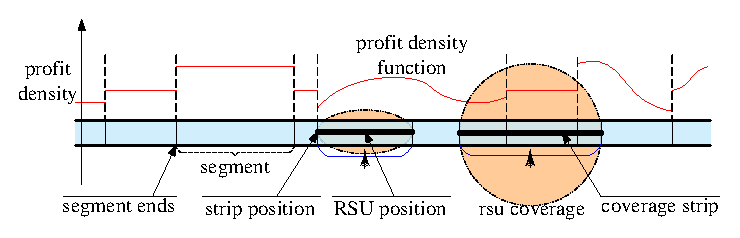
\includegraphics[width=0.48\textwidth]{rsu_roadline.eps}}
\caption{An example of the road line of a one-dimensional RDP problem.}
\label{fig_roadline}
\end{figure}

For a segment $e$ with ends $x_{e,0}$ and $x_{e,1}$, its profit density function $f_{e,w}(x)$ can be expressed as a function in coordinate system $(x,w)$ as shown in Eq.(\ref{eqn_pdf1d}).

\begin{equation}
\label{eqn_pdf1d}
f_{e,w}(x){\mathop{=}\limits^{\text{def}}}\left\{
\begin{array}{ll}
g_{e}(x), \hspace{3mm}&x{\in}[x_{e,0},x_{e,1}]\\
0,&x{\notin}[x_{e,0},x_{e,1}]
\end{array}
\right.
\end{equation}

If the road line consists of $L$ segments, then their profit density functions can be combined into one function as described in Eq.(\ref{eqn_pdfwhole}), which can then be regarded as the profit density function of the whole road line. Here $e_{e,i}$, $i{\in}\{0,1,\ldots,L\}$, are segment ends, and they satisfy $x_{e,i{-}1}{<}x_{e,i}$. Function $g_{e,i}(x)$ can be any non-negative differentiable function, whereas the whole function $g_e(x)$ is not required to be continuous at the segment ends. Such a $L$-segment piecewise differentiable function is general enough to describe any practical profit density functions. The differentiable assumption indeed is not a restriction, since that for any function with some non-differentiable at some points, we can split it into more segments at these non-differentiable points. This operation leads to a piecewise differentiable function with more segments.

\begin{equation}
\label{eqn_pdfwhole}
f_{e,w}(x){{:}w{=}}g_e(x){=}\hspace{-1mm}\left\{
\begin{array}{ll}
\hspace{-1mm}g_{e,0}(x){:=}0, &\hspace{-2mm}x{\in}({-}inf,x_{e,0})\\
\hspace{-1mm}g_{e,1}(x), &\hspace{-2mm}x{\in}[x_{e,0},x_{e,1}]\\
\hspace{-1mm}\ldots, &\hspace{-2mm}\ldots\\
\hspace{-1mm}g_{e,L}(x), &\hspace{-2mm}x{\in}(x_{e,L{-}1},x_{e,{L}}]\\
\hspace{-1mm}g_{e,L{+}1}(x){:=}0,&\hspace{-2mm}x{\in}(x_{e,L},inf)\\
\end{array}
\right.
\end{equation}

As shown in Fig.\ref{fig_roadline}, in one-dimensional RDP problem, whatever shape the coverage of a RSU has, its actual effect on covering the road line is equivalent to a line strip. The strip's length equals the length of the road line in the coverage. To maximize profit, the strip with maximum possible length should be used. For a circular coverage, the maximum length of the coverage strip equals the coverage's diameter, and the RSU should be placed at road side. Hence, the one-dimensional RDP problem is indeed to find the positions of a given number of RSUs along the road line such that accumulated profits of road parts covered by these RSUs are maximized.

In the following text, the concept \textbf{strip} is used to represent the effective coverage of a RSU on the road line, and the concept \textbf{strip length} means the length of the strip, which is denoted as $d$. If a strip covers a road segment of $[x,x{+}d]$, then we say that the strip is at $x$. For a RSU with circular coverage region of radius $r{=}d/2$, "place the strip at $x$" has the same meaning as "place the RSU at $x{+}r$". In the following text, $x$ is used as strip position by default, and $B(G(V,E),x{+}r,r,1)$ is abbreviated to $B(x)$.

\subsection{Comparison of Our RDP Problem with GSC and WMC}
Our RDP problem here looks similar to the well known Geometric Set Cover (GSC) problem \cite{WikiGSC} and the Weighted Maximum Coverage (WMC) problem\cite{WikiWMC}.

The GSC problem is the special case of the set cover problem in geometric settings\cite{WikiGSC}. The input is a range space $\Sigma{=}(X,\mathcal{R})\}$ where $X$ is a universe of points in $\mathbb{R}^{d}$ and $\mathcal{R}$ is a family of subsets of $X$ called regions, defined by the intersection of $X$ and geometric shapes such as disks and axis-parallel rectangles. The goal is to select a minimum-size subset $\mathcal{C}\subseteq{\mathcal{R}}$ of regions such that every point in the universe $X$ is covered by some range in $\mathcal{C}$.

Although looks similar, Our RDP problem and the GSC problem are different: (1)what should be covered in the GSC problem are some discrete points in $\mathbb{R}^{d}$, whereas they are curves with non-uniform weight densities in the RDP problem; (2)the objective of the GSC problem is to cover all given discrete points with minimum number of regions, whereas the objective of the RDP problem is to obtain maximum coverage profits with a given number of regions with given shapes and sizes. In the one-dimensional case, where $X$ contains points on the real line and $\mathcal{R}$ is defined by intervals, the GSC problem can be solved in polynomial time using a simple greedy algorithm. In higher dimensions where $d{\geq}2$, the GSC problem is known to be NP-complete even for simple shapes, i.e., when $\mathcal{R}$ is induced by unit disks or unit squares \cite{Fowler1981}.

The WMC problem is the weighted version of the maximum coverage (MC) problem. MC problem is also called as max k-cover problem\cite{Nemhau1978}. In the WMC problem, we are given a collection of elements with weights, several sets and a number $n$, the task is to select $n$ sets such that total weights of the elements in these sets are maximized. The WMC problem is NP-hard, and cannot be approximated within $1{-}{\frac {1}{e}}{+}o(1){\approx}0.632$ under standard assumptions\cite{WikiWMC}.

Our RDP problem can be regarded as the geometric extension of the maximum coverage (MC) problem. Although no proofs were found, we suspect that our RDP problem may be at least as hard as the GSC problem and the WMC problem. We also suspect that the one-dimensional RDP problem is also intractable, and we have't found existing works that solve the one-dimensional RDP problem. Our understanding even to the new one-dimensional RDP problem is still much lack.

\section{Properties of One-Dimensional RDP problem}
\label{sec_analysis}
\subsection{One-Dimensional RDP problem with One RSU}

For a one-dimensional RDP problem of one RSU with radius $r{=}d/2$, if the profit density function of the road line is a $L$-segment piecewise differentiable function, and if $x_{e,L}{-}x_{e,0}{\leq}d$, then it is easy to notice that all $x{\in}[x_{e,0}{+}r,x_{e,{L}}{-}r]$ are optimal solutions with the same profit. Hence, we will omit this trivial case in later analyses.

For optimal solutions of one-dimensional RDP problem with one RSU, we have the following Lemma \ref{lemma_1rsu_pcnt}. For expression clarity, we define several sets as in Eq.(\ref{eq_setdef_1}). Here $g_{e,{i{+}1}}(x_{e,i}^{+})$ represents the limit of $g_e(x)$ as $x$ infinitely approaches to $x_{e,i}$ from the right side, $g'_{e}(x)$ is the derivative of $g_{e}(x)$ with respect to $x$. $g'_{e,{i{+}1}}(x_{e,i}^{+})$ represents the limit of $g'_{e,{i{+}1}}(x)$ as $x$ infinitely approaches to $x_{e,i}$ from the right side. $g'_{e,i}(x_{e,i}^{-})$ represents the limit of $g'_{e,i}(x)$ as $x$ infinitely approaches to $x_{e,i}$ from the left side. Other symbols are defined similarly. It is easy to notice that the positions in $X_\text{cand}(d)$ are all local maximum points.

\begin{equation}
\label{eq_setdef_1}
\begin{array}{rl}
%%%%
X_\text{dif}(d){\mathop{=}\limits^{\text{def}}}
&\left\{
x|\substack{g_{e}(x{+}d){=}g_{e}(x),g'_{e}(x{+}d){-}g'_{e}(x){\leq}0,\\
x{\in}[x_{e,0}, x_{e,L}{-}d]}
\right\};\\
%
X_\text{moveL1}(d){\mathop{=}\limits^{\text{def}}}
&\left\{
x |g_e((x{+}d)^{-}){>}g_e(x^{-}),x{\in}[x_{e,0}, x_{e,L}{-}d]
\right\};
\\
%
X_\text{moveL2}(d){\mathop{=}\limits^{\text{def}}}
&\{
x |
\substack{g_e((x{+}d)^{-}){=}g_e(x^{-}),\\
g'_e((x{+}d)^{-}){\geq}g'_e(x^{-}),x{\in}[x_{e,0}, x_{e,L}{-}d]}
\};
\\
%
%
X_\text{moveR1}(d){\mathop{=}\limits^{\text{def}}}
&\left\{
x |g_e((x{+}d)^{+}){<}g_e(x^{+}),x{\in}[x_{e,0}, x_{e,L}{-}d]
\right\};
\\
%
X_\text{moveR2}(d){\mathop{=}\limits^{\text{def}}}
&\left\{
x |
\substack{g_e((x{+}d)^{+}){=}g_e(x^{+}),\\
g'_e((x{+}d)^{+}){\leq}g'_e(x^{+}),x{\in}[x_{e,0}, x_{e,L}{-}d]}
\right\};
\\
%
X_\text{moveL}(d){\mathop{=}\limits^{\text{def}}}&X_\text{moveL1}(d){\cup}X_\text{moveL2}(d);
\\
%
X_\text{moveR}(d){\mathop{=}\limits^{\text{def}}}&X_\text{moveR1}(d){\cup}X_\text{moveR2}(d);
\\
%
X_\text{move}(d){\mathop{=}\limits^{\text{def}}}&X_\text{moveL}(d){\cap}X_\text{moveR}(d);
\\
%
X_\text{cand}(d)
{\mathop{=}\limits^{\text{def}}}
&X_\text{move}(d);
\end{array}
\end{equation}


\begin{lemma}
\label{lemma_1rsu_pcnt}
For a one-dimensional RDP problem of one RSU with strip length $d$, if the profit density function of the road line is $L$-segment piecewise differentiable, and if $x_{e,L}{-}x_{e,0}{>}d$, then all optimal strip positions must be in set $X_\text{cand}(d)$.
\end{lemma}

\begin{IEEEproof}
The profit $B(x)$ of placing the strip at $x$ can be expressed as Eq.(\ref{eq_rdp1d_profit}) by using Eq.(\ref{eqn_modelbenefit}).

\begin{equation}
\label{eq_rdp1d_profit}
B(x){=}{\int}_{x}^{x{+}d}g_e(s)\text{d}s
\end{equation}

To determine the properties that optimal positions of the strip should have, we consider the following two cases depending on whether the ends of the strip are at segment ends.

\begin{itemize}

\item \textbf{Case 1: Neither ends of the strip are at segment ends}.

In this case, we conduct analyses in the following three subcases. Here we define function $id(x){\mathop{=}\limits^{\text{def}}}\{i|x{>}x_{e,i}, x{\leq}x_{e,i{+}1}\}$ for expression clarity.

\begin{itemize}
\item \textbf{Subcase 1: $id(x{+}d){=}id(x)$}.

In this case, Eq.(\ref{eq_rdp1d_profit}) can be calculated as Eq.(\ref{eq_rdp1d_c1_s1_1}).

\begin{equation}
\label{eq_rdp1d_c1_s1_1}
B(x){=}{\int}_{x}^{x{+}d}g_{e,id(x)}(s)\text{d}s
\end{equation}

Differentiate $B(x)$ with respect to $x$, we obtain

\begin{equation}
\label{eq_rdp1d_c1_s1_2}
\frac{\text{d}(B(x))}{\text{d}x}{=}g_{e,id(x)}(x{+}d){-}g_{e,id(x)}(x)
\end{equation}

\item  \textbf{Subcase 2: $id(x{+}d){=}id(x){+}1$}.

In this case, Eq.(\ref{eq_rdp1d_profit}) can be calculated as Eq.(\ref{eq_rdp1d_c1_s2_1}).

\begin{equation}
\label{eq_rdp1d_c1_s2_1}
\begin{array}{rl}
{\int}_{x}^{x{+}d}g_e(x)dx{=}&\hspace{-3mm}{\int}_{x}^{x_{e,id(x){+}1}}g_{e,id(x)}(s)\text{d}s\\
&\hspace{-3mm}{+}{\int}_{x_{e,id(x{+}d)}}^{x{+}d}g_{e,id(x{+}d)}(s)\text{d}s
\end{array}
\end{equation}

Differentiate $B(x)$ with respect to $x$, we obtain
\begin{equation}
\label{eq_rdp1d_c1_s2_2}
\begin{array}{l}
\frac{\text{d}(B(x))}{\text{d}x}{=}g_{e,id(x{+}d)}(x{+}d){-}g_{e,id(x)}(x)
\end{array}
\end{equation}

\item \textbf{Subcase 3: $id(x{+}d){>}id(x){+}1$}.

In this case, Eq.(\ref{eq_rdp1d_profit}) can be calculated as Eq.(\ref{eq_rdp1d_c1_s3_1}).

\begin{equation}
\label{eq_rdp1d_c1_s3_1}
\begin{array}{rl}
{\int}_{x}^{x{+}d}g_e(s)\text{d}s{=}&\hspace{-3mm}{\int}_{x}^{x_{e,id(x){+}1}}g_{e,id(x)}(s)\text{d}s\\
&\hspace{-6mm}{+}\mathop{\sum}\limits_{i{=}id(x){+}1}^{id(x{+}d){-}1}
{\int}_{x_{e,i}}^{x_{e,{i{+}1}}}g_{e,i}(s)\text{d}s\\
&\hspace{-6mm}{+}{\int}_{x_{e,id(x{+}d)}}^{x{+}d}g_{e,id(x{+}d)}(s)\text{d}s
\end{array}
\end{equation}

Differentiate $B(x)$ with respect to $x$, we obtain
\begin{equation}
\label{eq_rdp1d_c1_s3_2}
{\frac{\text{d}(B(x)))}{\text{d}x}}{=}g_{e,id(x{+}d)}(x{+}d){-}g_{e,id(x)}(x)
\end{equation}

In whichever of the three cases above, the derivative of $B(x)$ with respect to $x$ can be expressed as
\begin{equation}
\label{eq_rdp1d_c1_4}
\begin{array}{rl}
\frac{\text{d}(B(x))}{\text{d}x}&{=}g_{e,id(x{+}d)}(x{+}d){-}g_{e,id(x)}(x)\\
&{=}g_{e}(x{+}d){-}g_{e}(x)
\end{array}
\end{equation}

Each $x$ that maximizes $B(x)$ must satisfy Eq.(\ref{eq_rdp1d_c1_5}). Such positions are in set $X_\text{dif}(d)$.

\begin{subequations}
\label{eq_rdp1d_c1_5}
\begin{eqnarray}
\frac{\text{d}(B(x))}{\text{d}x}&{=}g_{e}(x{+}d){-}g_{e}(x){=}0;
\label{eq_rdp1d_c1_5_1}\\
\frac{\text{d}^2(B(x))}{\text{d}x^2}&{=}g'_{e}(x{+}d){-}g'_{e}(x){\leq}0;
\label{eq_rdp1d_c1_5_2}
\end{eqnarray}
\end{subequations}

\end{itemize}

\item \textbf{Case 2: One or two ends of the strip are at segment ends}.

In this case, either $x$ or $x{+}d$ or both of them are at segment ends, and the derivatives at these ends do not exist. The analyzing method used in case 1 is not applicable. However, we can analyze in another way as follows. For a strip at $x$ that maximizes $B(x)$, it must satisfy that moving the strip toward left or right for an infinitely small step should both decreases or at least not increases the profit of the strip.

For the case of moving left, the requirement of not increasing the profit leads to Eq.(\ref{eq_rdp1d_c2_1}), which leads to $X_\text{moveL}(d)$.

\begin{subequations}
\label{eq_rdp1d_c2_1}
\begin{eqnarray}
g_e((x{+}d)^{-}){>}g_e(x^{-});&
\label{eq_rdp1d_c2_1_1}\\
g'_e((x{+}d)^{-}){\geq}g'_e(x^{-}),& \hspace{-2mm}\text{if }g_e((x{+}d)^{-}){=}g_e(x^{-});
\label{eq_rdp1d_c2_1_2}
\end{eqnarray}
\end{subequations}

For the case of moving right, the requirement of not increasing the profit leads to Eq.(\ref{eq_rdp1d_c2_2}), which leads to $X_\text{moveR}(d)$.

\begin{subequations}
\label{eq_rdp1d_c2_2}
\begin{eqnarray}
g_e((x{+}d)^{+}){<}g_e(x^{+});&
\label{eq_rdp1d_c2_2_1}\\
g'_e((x{+}d)^{+}){\leq}g'_e(x^{+}),&\hspace{-2mm}\text{if }g_e((x{+}d)^{+}){=}g_e(x^{+});
\label{eq_rdp1d_c2_2_2}
\end{eqnarray}
\end{subequations}

Since that $x$ that maximizes $B(x)$ should satisfy both Eq.(\ref{eq_rdp1d_c2_1}) and Eq.(\ref{eq_rdp1d_c2_2}), all such $x$ must be in set $X_\text{move}(d){=}X_\text{moveL}(d){\cap}X_\text{moveR}(d)$.

\end{itemize}

Combining above two cases, we obtain that all $x$ maximizing $B(x)$ must be in set $X_\text{dif}(d){\cup}X_\text{move}(d)$. Furthermore, we can notice that each $x{\in}X_\text{dif}(d)$ must also satisfy both Eq.(\ref{eq_rdp1d_c2_1_2}) and Eq.(\ref{eq_rdp1d_c2_2_2}), hence we have $X_\text{dif}(d){\subseteq}(X_\text{moveL2}{\cap}X_\text{moveR2}){\subseteq}X_\text{move}$. As a result, we have $X_\text{dif}(d){\cup}X_\text{move}(d){=}X_\text{move}(d)$. The positions in $X_\text{move}(d)$ are called as candidate positions for the strip. To make symbols more meaningful, we define the set $X_\text{cand}(d)$ in Eq.(\ref{eq_setdef_1}) as an alias of $X_\text{mode}(d)$. The Lemma follows.
\end{IEEEproof}

Using Lemma \ref{lemma_1rsu_pcnt}, we can obtain the optimal positions of the RSU directly by (1) calculating $B(x)$ for all $x$ in $X_\text{cand}(d)$; (2) get the $x$ with maximum $B(x)$. The set $X_\text{cand}(d)$ may contain continuous regions in form of $[x_1,x_2]$, and thus the size of $X_\text{cand}(d)$ can be infinite. In this case, we can let $X_\text{cand}(d)$ contain only the end points of such regions, and then get the $x$ with maximum $B(x)$. If the $x$ obtained in this way is originally an end point of a region, then any position in the corresponding region will also be an optimal position.

\subsection{One-Dimensional Problem with Multiple RSUs}

If the total length of the RSUs' coverages is not smaller than the length of the road line, an obvious optimal solution is to place the strips along the road line such that the whole road is completed covered by the union of the strips. There may be many such optimal solutions. In later text, we omit this trivial case and focus on the normal non-trivial case. In the pseudo code of our algorithm in later text, code lines corresponding to the trivial case are also omitted.

When there are multiple RSUs, if the distance between two RSUs is smaller than the sum of their coverage radii, then the coverages of the two RSUs will overlap each other, or in other words, the corresponding strips overlap with each other. If there are overlapped strips in a solution, then we call it an overlapped solution, otherwise a non-overlapped solution. Maximizing each strip's profit may help to maximize the total profit of a solution, but the overall profit of overlapping strips are not independent, i.e., covering a road segment already covered by other strips brings no benefit. Helpfully, the one-dimensional RDP problem has the property in Lemma \ref{lemma_opt_nonlap}, which enables us to design efficient algorithms.

\begin{lemma}
\label{lemma_opt_nonlap}
For any one-dimensional RDP problem with multiple RSUs, there must be non-overlapped optimal solutions.
\end{lemma}

\begin{IEEEproof}
For any overlapped solution of a RDP problem instance, we can obtain a non-overlapped solution by stretching apart the overlapped strips meanwhile guaranteeing that the road segments covered by the overlapped solution are still covered by the non-overlapped solution. Thus, the profit of the non-overlapped solution must be not smaller than that of the overlapped solution. This property also applies to overlapped optimal solutions. Hence, if there are optimal solutions where strips overlap, then we must can obtain a new non-overlapped solution meanwhile it is optimal. The Lemma follows.
\end{IEEEproof}

In a non-overlapped solution, some strips may be adjacent to each other. By the adjacency relations, the strips in a solution form several groups, where the strips in each group are adjacent one-by-one, whereas the strips in different groups are separated. For a strip group contains $m$ strips, assume that the strips from left to right in the group have length $d_1,d_2,\ldots,d_{m}$, then we can regard the strip group as a virtual strip $s_{v}$ with length $d_{v}{=}\sum_{j{=}1}^{m}d_j$. For expression clarity, we can also regard an isolated strip as a virtual strip which has only one strip. If the virtual strip $s_{v}$ is placed at $x$, then the positions of the strips in the virtual strip are also determined, where the $k$-th strip is placed at $x_k{=}x{+}\sum_{j{=}1}^{k{-}1}(d_j)$, $1{\leq}k{\leq}m$. We denote the position set $\{x_1,x_2,\ldots,x_{m}\}$ as $X_\text{VS}(d_{v},x)$. Given a RDP problem instance with $n$ different RSUs, we denote the set of all possible lengths of the virtual strips as $S_\text{LVS}$. Then we define a set of positions $X_{\text{cand},n}\mathop{=}\limits^{\text{def}}\cup_{d{\in}S_\text{LVS}}(\cup_{x{\in}X_\text{cand}(d)}(X_\text{VS}(d,x)))$.

It is obvious that swapping positions of the strips in a virtual strip dose not change the overall profit of the virtual strip. Hence, if a virtual strip can be transformed to another virtual strip by only rearranging the sequences of the strips, then we regard that \textbf{the two virtual strips are identical}. Given two solutions, if the virtual strips in one solution have a one-to-one identical relation with the virtual strips in the other solution, then we regard that \textbf{the two solutions are identical}. With these concepts and definitions, we have the following lemma.

\begin{lemma}
\label{lemma_opt_candset}
For any one-dimensional RDP problem with $n$ RSUs having different coverage diameter, for any non-overlapped optimal solution, there must be an identical solution which is also optimal and the positions of the strips in this solution are all in set $X_{\text{cand},n}$.
\end{lemma}

\begin{IEEEproof}
We will prove it by contradiction. Assume that there is an optimal solution where positions of some strips are not in set $X_{\text{cand},n}$. These strips may form virtual strips by the adjacency relations. For any of these virtual strips, we assume that its length is $d$, then we must have $d{\in}S_\text{LVS}$. According to Lemma \ref{lemma_1rsu_pcnt}, the position $x$ of this virtual strip must be in $X_\text{cand}(d)$. Otherwise, we can increase the profit of the virtual strip by moving the virtual strip as a whole toward left or right, which contradicts with the assumption that this solution is optimal. As a result, this virtual strip must have an identical virtual strip where the positions of the strips in this later virtual strip must all be in set $X_\text{cand}(d)$. Similarly, there must be a solution with strip positions all in $X_\text{cand}(d)$ meanwhile  it is identical to the optimal solution. The lemma follows.
\end{IEEEproof}

If $X_{\text{cand},n}$ contains continuous regions, then it can be treated using the method applied to $X_{\text{cand}}(d)$ in the previous section.

If the strips have different lengths, then $|S_\text{LVS}|$ can be as larger as $2^n$, and the number of all possible different combinations of virtual strips can roughly be expressed as $\sum_{i{=}1}^{n}\frac{i^{n{-}1}{-}(i{-}1)^n}{(i{-}1)!}$.

To search for an optimal solution for a RDP problem with multiple RSUs, a straightforward way is to traverse all possible solutions. To do so, profits of all possible solutions may need to be checked thoroughly, where each solution consists of a combination of several virtual strips, and each virtual strip $s_{v}$ has its own corresponding set $X_\text{cand}(d_{v})$. According to Lemma \ref{lemma_opt_nonlap}, we need only to consider non-overlapped solutions. However, when there are multiple RSUs, if the strips have different lengths, then $|S_\text{LVS}|$ can be as larger as $2^n$, and the number of all possible different combinations of virtual strips can roughly be expressed as $\sum_{i{=}1}^{n}\frac{i^{n{-}1}{-}(i{-}1)^n}{(i{-}1)!}$. Thus, the number of possible solutions may be prohibitively large to be tackled. Contrastively, if all the strips have the same length, then we have $S_\text{LVS}{=}n$, and the number of all possible different combinations of virtual strips can roughly be expressed as $2^{n{-}1}$.  Thus, the one-dimensional RDP problem with identical RSUs is possibly more tractable. In later text, we focus on the later problem where all strips have length $d$. Although greedy or heuristic algorithms can be used to find quasi-optimal solutions, it is non-trivial to find an optimal solution.

\subsection{One-Dimensional Problem with Multiple Identical RSUs}
\label{sec_analysis_identical}
If all strips have the same length $d$, then each possible position $x$ of a virtual strip consisting of $m$ strips must be in set $X_\text{cand}(m{*}d)$. This $x$ actually corresponds to a list $[x,x{+}d,\ldots,x{+}(i{-}1)d]$, which are the positions of the strips in the virtual strip. Using notation $X{+}d\mathop{=}\limits^{\text{def}}\{x{+}d|x{\in}X\}$, the set of all candidate positions of strips determined by $X_\text{cand}(m{*}d)$ can be expressed as $X_\text{cand}(m,d){=}\mathop{\cup}\limits_{i{=}0}^{m{-}1}(X_\text{cand}(m{*}d){+}i{*}d)$, so we have $|X_\text{cand}(m,d)|{=}m{*}|X_\text{cand}(m{*}d)|$. Here $|s|$ denotes the size of set $s$. Making a symbol definition $X_\text{cand,c}(i,d)\mathop{=}\limits^{def}\mathop{\cup}\limits_{j{=}1}^{i}X_\text{cand}(j,d)$, the set of possible positions of all strips corresponding to all possible virtual strips is indeed $X_\text{cand,c}(n,d)$. We have $|X_\text{cand,c}(n,d)|{\leq}\mathop{\sum}_{i{=}1}^{n}(i{*}|X_\text{cand}(i{*}d)|)$. If $|X_\text{cand}(i{*}d)|=|X_\text{cand}((i{+}1){*}d)|{=}N$, $i{\in}\{1,2,\ldots,n{-}1\}$, then we have $|X_\text{cand,c}(n,d){\leq}\frac{n(n{+}1)}{2}N$. However, if most road segments have constant profit density function, Eq.\ref{eq_setdef_1} implies that most elements in $X_\text{cand}(i,d)$ are also elements of $X_\text{cand}(i{+}1,d)$. Thus, we can roughly assume that $X_\text{cand}(i,d){\subseteq}X_\text{cand}(i{+}1,d)$. As a result, $|X_\text{cand,c}(n,d)|{\approx}n{*}X_\text{cand}(1,d)|{=}\mathcal{O}(nL)$.

Each position in $X_\text{cand,c}(n,d)$ is a candidate position for a strip, and the ends of all the strips with position in $X_\text{cand,c}(n,d)$ divides the whole road line into small pieces, later we call these pieces as \textbf{slices}.

With these preparations, the main work to solve a one-dimensional RDP problem is actually to select the positions of $n$ non-overlapped strips from the set $X_\text{cand,c}(n,d)$ such that the overall profit of these selected strips is maximum.

For a one-dimensional RDP problem with multiple identical RSUs, the overlap relationships among the strips with positions in $X_\text{cand,c}(n,d)$ can be expressed as a weighted graph. In this graph, each node represents a candidate strip with its corresponding position, the weight of the node is the profit of the strip. If two strips are overlapped, a link is inserted between the two corresponding nodes. This graph is indeed the interval graph of the strips in $X_\text{cand,c}(n,d)$.

With this graph, the RDP problem is equivalent to the problem of finding $n$ independent nodes with maximum total weight. This problem has relation to a well known Non-deterministic Polynomial Complete(NPC) problem in graph theory, named Maximum Weighted Independent Set (MWIS)\cite{WikiIS}. In MWIS, the number of nodes to be selected is a variable to be solved. Different from the MWIS problem, the number of nodes to be selected here is a given parameter.

\section{Greedy based Approximate Algorithms to the RDP Problem with Heterogenous RSUs}
\label{sec_diffrsu}
Suspecting that finding an optimal solution for the one-dimensional RDP Problem with multiple RSUs of different radii is intractable, greedy-based approach is a natural way for obtaining approximate solutions. We propose two greedy-based approximate algorithms Greedy2P3 and Greedy2P3E. According to Lemma \ref{lemma_opt_nonlap}, our algorithms only consider non-overlapped solutions, i.e., solutions where the strips are non-overlapped.

\subsection{Greedy2P3 Algorithm}

Pseudo code of the Greedy2P3 algorithm is shown in Algorithm \ref{Alg_Greedy2P3}. In this code, structural variable $roadNet$ contains raw information about the problem, structural variable $dataMat$ contains information such as list of candidate strip positions, list of strip profits, strip overlap information. $dataMat$ is generated by function $\verb"getDataMatfromRoad"(roadNet)$. Function $\verb"getPosMaxFree"(dataMat,posList,dList(i))$ return the strip with maximum profit among all strips uncovered by the strips in $optList$. Function $\verb"sortDescending"(dList)$ returns the sorted list of the diameters of the RSUs in descending order. Function $\verb"UpdateRoadNet"(dataMat,dList(i))$ updates road line information, i.e, resets the profit density function of the road parts covered by the strip at $dList(i)$ to 0, and obtain the set $X_{cand,1}(dList(i))$ corresponding to the updated road line using Lemma \ref{lemma_1rsu_pcnt}.

\begin{algorithm}[htb]
\caption{The Greedy2P3 Algorithm}
\begin{algorithmic}[1]\label{Alg_Greedy2P3}
    \REQUIRE $n$: number of RSUs to be deployed;\\
    $roadNet$: road network;\\
    $dList$: the list of the diameters of the RSUs;
    \ENSURE $posList$: the list of the selected strips;\\
     $maxProfit:$the profit of the best solution found;
    \STATE $posList{=}[\hspace{1mm}]$; $maxProfit{=}0$;
    \STATE $dList{=}\verb"sortDescending"(dList)$;
    \STATE $dataMat{=}\verb"getDataMatfromRoad"(roadNet)$;
    \FOR {$i{=}1:n$}
        \STATE $[dataMat]{=}\verb"UpdateRoadNet"(dataMat,dList(i))$;
        \STATE $[pos,val]{=}\verb"getPosMaxFree"(dataMat,posList,dList(i))$;
        \STATE $posList{=}[posList,pos]$;
        \STATE $maxProfit{=}maxProfit{+}val$;
    \ENDFOR
    \STATE return $[posList,maxProfit]$;
\end{algorithmic}
\end{algorithm}

\subsection{Greedy2P3E Algorithm}

In Greedy2P3, function $\verb"getPosMaxFree"(dataMat$, $optList,dList(i))$ only considers strips non-overlap with the strips in $optList$, which neglects possible better strips. Such an example is shown in Fig.\ref{fig_rsu_example2p3} in Section \ref{sec_ratio2p3}. In this instance, $n{=}3$, and the whole road line is divided into 11 slices. The symbol in a slice indicates the profit obtained by covering the slice. Here $a$,$b$ are non-negative constants and satisfy $a{>}b$, and $\varepsilon$ is a non-negative constant which can be infinitely small. For this instance, Greedy2P3 will select three strips $cg_1$, $cg_2$, and $cg_3$ one by one. However, it is easy to notice that the strip $cg'_3$ is a better option when selecting the third strip. This instance implies that, Greedy2P3 may neglect some simple chances that lead to better profit. This motivates us to propose Greedy2P3E. Greedy2P3E exploits such chances when selecting new strips, and then after selecting enough strips, the strips are moved so as to obtain a final better non-overlapped solution.

\begin{algorithm}[htb]
\caption{Greedy2P3E Algorithm}
\begin{algorithmic}[1]\label{Alg_Greedy2P3E}
    \REQUIRE $n$: number of RSUs to be deployed;\\
    $roadNet$: road network;\\
    $dList$: the list of the diameters of the RSUs;
    \ENSURE $posList$: the list of the selected strips;\\
     $maxProfit:$the profit of the best solution found;
    \STATE $posList{=}[\hspace{1mm}]$; $maxProfit{=}0$;
    \STATE $dList{=}\verb"sortDescending"(dList)$;
    \STATE $dataMat{=}\verb"getDataMatfromRoad"(roadNet)$;
    \FOR {$i{=}1:n$}\label{stage1begin}
        \STATE $[dataMat]{=}\verb"UpdateRoadNet"(dataMat,dList(i))$;
        \STATE [$pos,addiVal$]{=}\verb"getPosMaxAddiProfit"(
        \STATE $dataMat,posList,dList(i)$);
        \STATE $posList{=}[posList,pos]$;
        \STATE $maxProfit{=}maxProfit{+}addiVal$;
    \ENDFOR \label{stage1end}
    \WHILE {isExist(overlapped strips in $posList$)}\label{stage2begin}
        \STATE [$ccs,n_{ccs}]{=}\verb"selContinueSegOverlap"(posList)$;
        \STATE $posList{=}\verb"solveOverlaps"(roadNet,posList,ccs,n_{ccs})$;
    \ENDWHILE \label{stage2end}
    \STATE $maxProfit{=}\verb"calProfit"(posList)$;
    \STATE \textbf{return} $posList,maxProfit$;
\end{algorithmic}
\end{algorithm}

The Greedy2P3E algorithm solves a RDP problem instance in two stages. Code lines \ref{stage1begin}-\ref{stage1end} forms Stage1, code lines \ref{stage2begin}-\ref{stage2end} forms Stage2. Stage1 is similar to Greedy2P3 except that function $\verb"getPosMaxFree"(\cdot)$ is replaced by function $\verb"getPosMaxAddiProfit"(\cdot)$. The latter function selects a strip with maximum additional profit. Additional profit of the strip represents the total profit of road part only covered by this strip, whereas the profits of the road part covered by previously selected strips are not considered.

If the solution obtained in Stage1 has overlapped strips, the additional Stage2 will be performed. In stage2, each overlapped strip set is replaced with a continuous non-overlapped strip set, where the left most strip in the overlapped strip set is kept unchanged, whereas all other strips in the overlapped strip set are extended towards right one by one. To be specific, function $\verb"selContinueSegOverlap"(posList)$ selects one overlapped strip set, and function $\verb"solveOverlaps"(\cdot)$ replaces the selected overlapped strip set with its corresponding continuous non-overlapped strip set.

\subsection{Property Analysis on the Algorithms}

\begin{lemma}
\label{lemma_greedybetter}
For any RDP problem instance, a solution found by Greedy2P3E must be not worse than one found by Greedy2P3.
\end{lemma}

\begin{IEEEproof}
Both algorithms select new strips repeatedly by selecting one in each loop. For the first two loops, the strips selected by Greedy2P3 and Greedy2P3E must be the same. In the later loops, it can be noted easily that the set of candidate strips inspected by function $\verb"getPosMaxAddiProfit"(\cdot)$ in Greedy2P3E must be a superset of that inspected by function $\verb"getPosMaxFree"(\cdot)$ in Greedy2P3P. Hence, the profit of the strip selected in Greedy2P3E must be not smaller than one selected in Greedy2P3. Therefore, total profit of solution found by Greedy2P3PE after Stage1 must be not smaller than one by Greedy2P3. Furthermore, the optional Stage2 in Greedy2P3E will replace overlapped solutions with a non-overlapped one, meanwhile guaranteeing that the profit of the non-overlapped solution is not smaller than that of the overlapped one. As a conclusion, the lemma follows.
\end{IEEEproof}

Although Greedy2P3 is not better than Greedy2P3E, we prove in later sections that Greedy2P3 has a tight constant approximation ratio for one-dimensional RDP problems with multiple RSUs of identical diameter, thus provides a lower bound for the approximation ratio of Greedy2P3E.

Running time of the greedy algorithms depends on $|X_\text{cand}(dList(i))|$ $(i{=}1,2,...,n)$. $|X_\text{cand}(dList(i))|$ depends on segment number $L$ of the whole road line. Eq.(\ref{eq_setdef_1}) implies that, if all segments have constant profit density function, then we have $|X_\text{cand}(dList(i))|{\leq}2{*}L$. Otherwise, $|X_\text{cand}(dList(i))|$ may be boundlessly large, but such cases are unusual in practice. Ignoring such less practical cases, we denote that $|X_\text{cand}(dList(i))|{=}N$. Then, for time complexity of the two algorithms, we have the following Lemma \ref{lemma_greedy_time}.

\begin{lemma}
\label{lemma_greedy_time}
Time complexity of Greedy2P3 and Greedy2P3E are both $\mathcal{O}(nN)$.
\end{lemma}

\begin{IEEEproof}
Main operation in the loop in Greedy2P3 is to obtain set $X_\text{cand}(dList(i))$, and calculates their corresponding profits. This operation requires time $\mathcal{O}(N)$. Function $\verb"getPosMaxFree"(\cdot)$ returns the best free strip in time $\mathcal{O}(N)$. Hence, each loop requires time $\mathcal{O}(N)$. The loop repeats $n$ times, hence total running time will be $\mathcal{O}(nN)$.
Stage1 of Greedy2P3E also has time complexity $\mathcal{O}(nN)$. Stage2 of Greedy2P3E can be completed in time $\mathcal{O}(n)$. Hence, time complexity of Greedy2P3E is $\mathcal{O}(nN){+}\mathcal{O}(n){=}\mathcal{O}(nN)$. The lemma follows.
\end{IEEEproof}

Greedy algorithms are approximate algorithms, which usually return approximate solutions. For a certain problem instance, the ratio of the profit of a solution returned by an approximate algorithm to that of an optimal solution is named \textbf{performance ratio} of the approximate algorithm with the given instance. For different problem instances, the performance ratio is usually different. In the literature, another concept of \textbf{approximation ratio} \cite{Kim2017,Li2014} is used to measure the approximation ability of approximate algorithms, which is defined as the minimum of all possible performance ratios.

\begin{lemma}
\label{lemma_greedy2p3e_ratio}
For approximation ratio of Greedy2P3E, denoted as $\alpha_\text{2P3E}$, we have $\alpha_\text{Greedy2P3E}{\geq}1{-}(\frac{n{-}1}{n})^n$.
\end{lemma}

\begin{IEEEproof}
Results in \cite{Nemhau1978} shows that, for max $n$-cover problem, if the profit function $f$ defined on the covers meets Eq.(\ref{eq_submod}), then the greedy algorithm, which iteratively selects the set that has the maximum additional profit, has an approximation ration of at least $1{-}(\frac{n{-}1}{n})^n$.
Obviously our deployment profit model ensures that the profit of strips in our RDP problem satisfies Eq.(\ref{eq_submod}). Furthermore, function $\verb"sortDescending"(dList)$ ensures that the strips are treated in descending order, so our Greedy2P3E algorithm works exactly greedily. Thus, the result about the approximation ratio also applies to Greedy2P3E. The lemma follows.
\end{IEEEproof}

\begin{equation}
\label{eq_submod}
\begin{array}{ll}
f(U){+}f(V){\geq}&f(U{\cup}V){+}f(U{\cap}V), \\
&U \text{and} V \text{are any covers};\\
f(\emptyset){=}0;&
\end{array}
\end{equation}

\section{Optimal Algorithm OptGreDyn for One-dimensional RDP Problem with identical RSUs}
\label{sec_algopt}

\subsection{Optimal Algorithm OptGreDyn}

According to Lemma \ref{lemma_opt_candset} and Lemma \ref{lemma_opt_nonlap}, set $X_\text{cand,c}(n,d)$ must contain at least one optimal solution. Thus, the task of the RDP problem is indeed to find a combination of $n$ different values of $x$ such that the corresponding strips are non-overlapped meanwhile their total profit is maximum. A straight forward way is by traversing all $\mathcal{O}((M)^n)$ possible combinations of strips, here $M$ represents $|X_\text{cand,c}(n,d)|$. As $M$ becomes much large, this approach will be very time consumptive.

For the one-dimensional RDP problem with multiple identical RSUs, we found the following property.

\begin{lemma}
\label{lemma_gredyn_property}
For the best strip $s_1$ in $X_\text{cand,c}(n,d)$, there must be an optimal non-overlapped solution that satisfies one of the two conditions:
(Cond1)the optimal solution contains $s_1$;
(Cond2)the optimal solution contains two other strips $s_2$ and $s_3$ such that $s_2$ and $s_3$ are non-overlapped with each other, but they all overlap with $s_1$.
\end{lemma}

\begin{IEEEproof}
We will prove by contradiction. According to Lemma \ref{lemma_opt_nonlap}, there must be non-overlapped optimal solutions. Assume that all these optimal solutions do not satisfy the two conditions. Then for each such optimal solution $S_1$, we can replace any one strip $s_4$ in the solution with strip $s_1$, thus obtain a new solution $S_2$. The assumption implies that $s_4$ non-overlap with $s_1$. Since that $s_1$ is the best one in $X_\text{cand,c}(n,d)$, we have
$B(S_2){-}B(S_1){=}B(s_1){-}B(s_4){\geq}0$. Hence, $S_2$ must also be an optimal solution, which satisfies Cond1, thus we have a contradiction. The lemma follows.
\end{IEEEproof}

We use $X$ to represent $X_\text{cand,c}(n,d)$ for expression brevity. For a strip $s_1$, we denote the set of the pairs $(s_2, s_3)$ satisfying cond2 as $C(s_1)$. Given $X$ and $n$, we use $\mathcal{S}(X,n)$ to denote the profit of an optimal solution, then Lemma \ref{lemma_gredyn_property} implies Eq.(\ref{eq_optdyn}). Here $X{-}s$ represents the set obtained from $X$ by removing all strips that overlap with strip $s$.

\begin{equation}
\label{eq_optdyn}
\begin{array}{ll}
\mathcal{S}(X,n){=}
\text{max}\left(
\substack{B(s_1){+}\mathcal{S}(X{-}s_1,n{-}1)),\\
\{B(s_2){+}B(s_3){+}\mathcal{S}(X{-}s_2{-}s_3,n{-}2)\}_{(s_2,s_3){\in}C(s_1)}}
\right)
\end{array}
\end{equation}

Eq.(\ref{eq_optdyn}) enable us an efficient optimal algorithm combing greedy and dynamic programming techniques, hence comes the name OptGreDyn. Its pseudo code is shown in Algorithm \ref{alg_OptGreDyn}. Function $\verb"getOptSol"(X,n)$ implements Eq.(\ref{eq_optdyn}). Function $\verb"getPosMaxFree"(X)$ returns the best strip. Function $\verb"sortProfitDesc"(X)$ sorts the strips in descending order of profit. Function $\verb"getStripPairCond2"(X,x)$ returns the set of $(s_2,s_3)$ pairs satisfy cond2. Here $B(x)$ denotes the profit of strip $x$.

\begin{algorithm}[htbp]
\caption{OptGreDyn Algorithm}
\begin{algorithmic}[1]
\label{alg_OptGreDyn}
    \REQUIRE $n$: number of RSUs to be deployed;\\
    $X$: abbreviation of $X_\text{cand,c}(n,d)$;\\
    $d$: length of each coverage strip;
    \STATE $[optList,maxP]{=}\verb"getOptSol"(X,n)$;
    \STATE \textbf{Function} $[sol]{=}\verb"getOptSol"(X,i)$
    \STATE $maxP{=}0$;
    \IF {$i{==}1$}
        \STATE $[x]{=}\verb"getPosMaxFree"(X)$;
        \STATE return $\{x,B(x)\}$;
    \ELSIF {$i{==}2$}
        \STATE $[xList]{=}\verb"sortProfitDescUpdate"(X)$;
        \FOR {$i{=}1{:}|X|$} \label{opt_case2_forbegin}
            \STATE $[optList,v]{=}\verb"getOptSol"(X{-}xList(i),i{-}1)$;
            \IF {$B(xList(i)){+}v{>}maxP$}
                \STATE $maxP{=}v+B(xList(i))$;
                \STATE $optList{=}[xList(i),optList]$;
            \ENDIF
            \IF {$B(xList(i)){<}v$}
                \STATE break;
            \ENDIF
        \ENDFOR \label{opt_case2_forend}
        \STATE return $\{optList,maxP\}$;
    \ELSE
        \STATE $[xList]{=}\verb"sortProfitDesc"(X)$; \label{opt_case3_begin}
        \STATE $[optList,v]{=}\verb"getOptSol"(X{-}xList(1),i{-}1)$;
        \IF {$B(xList(1)){+}v{>}maxP$}
            \STATE $maxP{=}B(xList(1)){+}v$;
            \STATE $optList{=}[xList(1),optList]$;
        \ENDIF
        \STATE $[\mathcal{C}]{=}\verb"getStripPairCond2"(X,xList(1))$;\label{opt_case3_pair}
        \FOR {$each (s_2,s_3){\in}C$}
            \STATE $[optList,v]{=}\verb"getOptSol"(X{-}s_2{-}s_3,i{-}2)$;
            \IF {$B(s_2){+}B(s_3){+}v{>}maxP$}
                \STATE $maxP{=}B(s_2){+}B(s_3){+}v$;
                \STATE $optList{=}[s_2,s_3,optList]$;
            \ENDIF
        \ENDFOR
        \STATE return $\{optList,maxP\}$; \label{opt_case3_end}
    \ENDIF
    \STATE \textbf{End Function}
\end{algorithmic}
\end{algorithm}


\begin{lemma}
\label{lemma_greedyn_optimal}
A solution obtained by the OptGreDyn algorithm must be optimal.
\end{lemma}

\begin{IEEEproof}
We prove it by mathematical induction. It is obvious that when $n{=}1$ and $n{=}2$, a solution found by OptGreDyn must be optimal. Now assume that it is also true for $n{=}i$ and $n{=}i{-}1$. Since that the code lines \ref{opt_case3_begin}-\ref{opt_case3_end} implement Eq.(\ref{eq_optdyn}), then using Lemma \ref{lemma_gredyn_property}, the solution obtained at line \ref{opt_case3_end} must be an optimal solution for $n{=}i{+}1$. The lemma follows.
\end{IEEEproof}

Assume that the average size of $\mathcal{C}$ obtained by code line \ref{opt_case3_pair} in OptGreDyn is $C$, the average number of loops executed in the for loop implemented by code lines \ref{opt_case2_forbegin}-\ref{opt_case2_forend} is $F$. We usually have $C{\ll}n^2N$, $F{\ll}n^2N$.

\begin{lemma}
\label{lemma_optgredyn_time}
Time complexity of OptGreDyn is $\mathcal{O}(C^{(n{-}2){/}2}F{+}M\text{log}(M))$ when $n{=}2{*}i$, and $\mathcal{O}(C^{(n{-}3){/}2}(C{+}F){+}M\text{log}(M))$ when $n{=}2{*}i{+}1$, where $i$ is an integer.
\end{lemma}

\begin{IEEEproof}
In the pseudo code of the OptGreDyn algorithm, function $\verb"sortProfitDesc"(X)$ is called in several code lines with slightly different $X$. Hence, in practical implementation, we can sort $X$ once and then reuse the sorted list later with some trivial updating operation. Thus, total time of all calls to function $\verb"sortProfitDesc"(X)$ can be assumed to be $T(s){=}\mathcal{O}(M\text{log}(M))$.

Denoting the running time of recursive iterations with $n$ as $T(n)$, we have $T(n){=}T(n{-}1){+}C{*}T(n{-}2)$. With $T(1){=}\mathcal{O}(1)$ and $T(2){=}F{*}T(1){=}\mathcal{O}(F)$, we obtain $T(2{*}i){=}\mathcal{O}(C^{i{-}1}F)$ and $T(2{*}i{+}1){=}\mathcal{O}(C^{i{-}1}(C{+}F))$.

Combining $T(s)$ and $T(n)$, the lemma follows.
\end{IEEEproof}

\subsection{Dynamic Limiting Technique}
\label{sec_dynlim}
Another possible approach to the one-dimensional RDP problem with multiple identical RSUs is called as dynamic limiting technique. This technique works in a depth-first exhaustively-search-like way, but tries to reduce search space size in the searching process by dynamically setting the lower limits of the orders of the strips that can be used to construct candidate solutions. Here the order of a strip is its index in the sorted list of the strips in $X_\text{cand,c}(n,d)$ sorted in descending order of profit. Assume that we use $t[1{:}n]\mathop{=}\limits^\text{def}[t_1, t_2,\ldots,t_n]$ to denote the order limits, then using the dynamic limiting technique, only the strips with orders smaller than $t_i$ can be selected as the $i$-th strip of a candidate solution. Further more, when all RSUs have identical diameter, swapping positions of the strips in a solution do not make a difference. Hence, we need only search through solutions where the $i$-th strip has order smaller than the $j$-th strip, $j{>}i$. Once a new candidate solution is constructed and checked for optimality, the limits $t[1{:}n]$ will be adjusted when possible for reducing search space size. The underlying idea for adjusting limits is simple and can be cleared in the example. Assume an instance of the RDP problem with $n{=}3$, if we find a candidate solution $s[1{:}3]{=}[1,3,7]$, then we can set $t[1{:}3]{=}[s[3]{-}2,s[3]{-}1,s[3]]{=}[5,6,7]$ by the fact that any candidate solution, where the order of the first element is at least 5, must have profit not greater than $B_o([1,3,7])$. Hence, we can omit all solutions with $s[1]{\geq}5$. Limits of other elements are determined similarly.

We have proposed an algorithm named as OptDynLim using the dynamic limiting technique. Simulations shows that OptDynLim is less efficient than OptGreDyn, so we just provide the idea here. In performance evaluation section, OptDynLim is used as a reference for other algorithms.

\section{Approximation Ratio of Greedy2P3 and Greedy2P3E when RSUs Having Identical Radii}
\label{sec_ratio2p3}
The approximation ratio of the Greedy2P3 algorithm to RDP problem with multiple identical RSUs is 2/3, and it is tight. Before proving this, we first make some definitions as follows.
\begin{itemize}
\item \textbf{Greedy solution and greedy strip}: a solution returned by our Greedy2P3 algorithm is called a greedy solution. The strips in a greedy solution are called as greedy strips.

\item \textbf{Optimal solution and optimal strip}: Solutions with maximum profit are called as optimal solutions. Here we only consider non-overlapped optimal solutions. The strips in an optimal solution are called as optimal strips.

\item \textbf{Overlapped strips and non-overlapped strips}: If the joint of the coverages of two strips is non-empty, we say that they are overlapped, otherwise they are non-overlapped. \textbf{Adjacent strips} are regarded as non-overlapped.

\item \textbf{Completely overlapped and partly overlapped}: For overlapped strips, there are two sub cases: if their coverages are identical, then they are completely overlapped, otherwise they are partly overlapped.

\item \textbf{Free strips}: Strips those are non-overlapped with other strips are called as free strips.

\item \textbf{direct connection, indirect connection, path}: For the pair of a greedy strip and an optimal strip, if the two strips are overlapped, we say that they have direct connection, or they are directly connected. For any two strips $c_1$ and $c_n$, if there is a list $[c_1,c_2,\cdots,c_n]$ such that $c_j$ and $c_{j{+}1}$ are directly connected, $j{\in}\{1,2,\cdots,n{-}1\}$, then we say that $c_1$ and $c_n$ are indirectly connected. This list is called a path. If two strips are either directly connected or indirectly connected with each other, we say that they are \textbf{connected} with each other.

\item \textbf{Strip cell and Cell style}: For analysis purpose, small set of connected strips with typical structure is called a cell. Respect to connection relationships as well as relative superiority of the strips in profit, cells are classified into cell styles.

\item \textbf{Stable, unstable, and invalid cell style}: If a cell style can actually exist without connecting to any other strips, we say that this style is stable. Otherwise, if a cell style can only exist by connecting to other strips, we say that it is unstable. Cell styles that could not actually exist is called invalid cell style.

\item \textbf{Strip group and group style}: For a set of connected strips, if the strips are not connected with other strips not belonging to the set, then such a strip set is called as a strip group. According to the structural characteristics and relative priority of the strips in profit, strips groups are classified into group styles.

\item \textbf{balanced group and unbalanced group}: A strip group with equal number of greedy strips and optimal strips is called a balanced group, otherwise it is a unbalanced group.

\item \textbf{Logic group and logic group style}: By logically rearranging (e.g, removing from or inserting into) strips in unbalanced groups, we can make unbalanced groups become balanced. Balanced groups obtained by using \textbf{logic rearrangement operations} are called as logic groups. In a logical group, we say that the newly logically inserted strip and the previously contained strips in the group are \textbf{logically connected}. Logic groups are classified into \textbf{logic group styles}.
\item \textbf{Greedy profit and optimal profit of a logic group}: For a logic group, the total profit of the greedy strips in the group is called the greedy profit of the group. Similarly, the total profit of the optimal strips are called as optimal profit of the group.

\end{itemize}

\textbf{Cell style, group style, and logic group style are all abstract concepts. They are category representations of cells, groups, and logic groups, respectively}.

The whole process for proving the approximation ratio of the Greedy2P3 algorithm can be roughly expressed in 5 steps as follows.
\begin{enumerate}[\textbf{Step}1:]
\item We totally identify 15 cell styles, and determine whether they are stable, unstable, invalid. (Refer to Appendix \ref{secApp_greedy_cs}).
\item Based on the properties of the cell styles, and using the fact that an unstable cell must join a group by connecting to stable cells through paths, we identify 8 group styles (Refer to Appendix \ref{secApp_greedy_gs}).
\item We make all unbalanced groups become balanced by using logic rearrangement operations. We identify 6 logic group styles (Refer to Appendix \ref{secApp_greedy_lgs}).
\item For each logic group style, we prove its performance ratio(Refer to Appendix \ref{secApp_greedy_lgspr}).
\item We prove the approximation ratio of the Greedy2P3 algorithm by combining performance ratios of the logic group styles, and show that it is tight by providing some problem instances which can approach this approximation ratio.
\end{enumerate}

The 6 logic group styles are shown in the sub figures in Fig.\ref{fig_rsu_logicgroup}. These logic group styles are denoted as $LGS_a$, $LGS_b$, $LGS_c$, $LGS_d$, $LGS_e$ and $LGS_f$, respectively. In these sub figures, a solid arrow represents direct connection between the two corresponding strips, whereas a dashed arrow represents logic connection. An arrow from strip $a$ to strip $b$ means $B(b){\geq}B(a)$, here $B(x)$ denotes the profit of strip $x$. A double ended arrow means that this arrow can have either direction. Parallel solid and dashed arrows between a pair of strips mean that the connection between the two strips can be either a direct connection or a logic connection.

\begin{figure}[ht]
\centering{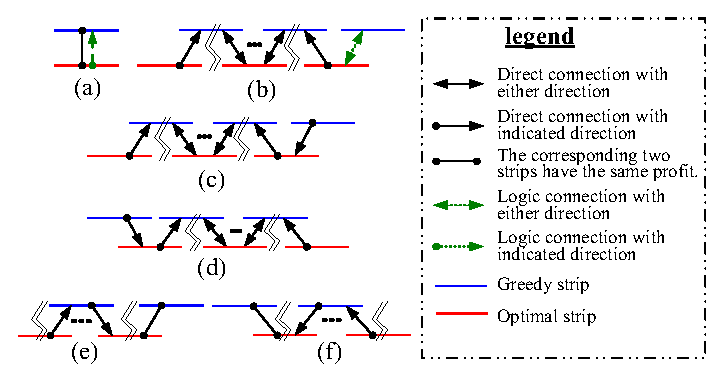
\includegraphics[width=0.48\textwidth]{rsu_logicgroupstyle.eps}}
\caption{Logic group styles.}
\label{fig_rsu_logicgroup}
\end{figure}

In the following text, we only provide the detailed prove process for step 5. Detailed process for other steps are given in Appendix \ref{secAppGreedy}.

\begin{theorem}
\label{lemma_greedy_approx_ratio}
The approximation ratio of the Greedy2P3 algorithm, denoted as $\alpha_\text{G2P3}$, is at least 2/3, and it is tight for $n{=}3{*}i$, here $i$ is any positive integer.
\end{theorem}

\begin{IEEEproof}
We will prove it by firstly showing that its performance ratio on any problem instance should be at least 2/3, and then showing that there are problem instances with performance ratio infinitely approach 2/3, thus the proof can be completed.

As shown in Appendix \ref{secAppGreedy}, for any instance of one-dimensional RDP problem with multiple identical RSUs, for any certain greedy solution and any non-overlapped optimal solution, the greedy strips and the optimal strips can must be grouped into logic groups of the 6 logic group styles. Without loss of generality, we assume that the numbers of logic groups of style $LGS_a$, $LGS_b$, $LGS_c$, $LGS_d$, $LGS_e$ and $LGS_f$,are $n(a)$, $n(b)$, $n(c)$, $n(d)$, $n(e)$ and $n(f)$, respectively.

For any logic group $LG_{a,i}$ of style $LGS_a$, we denote its greedy profit and optimal profit as $B_\text{G2P3}(a,i)$ and $B_\text{Opt}(a,i)$, respectively. Notations for other logic groups are defined similarly. About the performance ratios of Greedy2P3 on logic groups of the 6 styles, results in section \ref{secApp_greedy_lgspr} shows that we have $\beta_\text{LGS}(b){\geq}2/3$, $\beta_\text{LGS}(c){\geq}2/3$, $\beta_\text{LGS}(d){\geq}2/3$, $\beta_\text{LGS}(e){\geq}1$ and $\beta_\text{LGS}(f){\geq}1$. Hence, the performance ratio of Greedy2P3 on the given problem instance, denoted as $\beta_\text{G2P3}$, can then be calculated as Eq.(\ref{eq_greedy2p3_1}), which shows that $\beta_\text{G2P3}{\geq}2/3$.

\begin{equation}
\label{eq_greedy2p3_1}
\begin{array}{rl}
\beta_\text{G2P3}{=}\frac{B_\text{G2P3}}{B_\text{Opt}}&{=}
\frac
{
\mathop{\sum}_{x{\in}\{a,b,c,d,e,f\}}
\left(
\mathop{\sum}_{i{=}1}^{n_x}B_\text{2P3}(x,i)
\right)
}
{
\mathop{\sum}_{x{\in}\{a,b,c,d,e,f\}}
\left(
\mathop{\sum}_{i{=}1}^{n_x}B_\text{Opt}(x,i)
\right)
}\\
&{\geq}
\frac
{
\mathop{\sum}_{x{\in}\{a,b,c,d,e,f\}}
\left(
\mathop{\sum}_{i{=}1}^{n_x}\beta_\text{LGS}(x)B_\text{Opt}(x,i)
\right)
}
{
\mathop{\sum}_{x{\in}\{a,b,c,d,e,f\}}
\left(
\mathop{\sum}_{i{=}1}^{n_x}B_\text{Opt}(x,i)
\right)
}\\
&{\geq}
\frac
{
\mathop{\sum}_{x{\in}\{a,b,c,d,e,f\}}
\left(
\mathop{\sum}_{i{=}1}^{n_x}2/3*B_\text{Opt}(x,i)
\right)
}
{
\mathop{\sum}_{x{\in}\{a,b,c,d,e,f\}}
\left(
\mathop{\sum}_{i{=}1}^{n_x}B_\text{Opt}(x,i)
\right)
}\\
&{=}2/3
\end{array}
\end{equation}

Now we will show that there are some RDP problem instances where the performance ratios of Greedy2P3 infinitely approach 2/3. Such an instance is shown in Fig.\ref{fig_rsu_example2p3}. In this instance, $n{=}3$, and the whole road line is divided into 11 slices. The symbol in a slice indicates the profit obtained by covering the slice. Here $a$,$b$ are non-negative constants, $\varepsilon$ is a non-negative constant which can be infinitely small. Without loss of generality, we assume that $a{>}b$. For this instance, it is easy to check that the strip set $\{co_1$, $co_2$, $co_3\}$ is its optimal solution, whereas the greedy solution will be $\{cg_1$, $cg_2$, $cg_3\}$. Performance ratio $\beta_\text{G2P3}$ of Greedy2P3 on this instance can be calculated as Eq.(\ref{eq_greedy2p3_2}), which shows that $\beta_\text{G2P3}{\rightarrow}2/3$ when $\varepsilon{\rightarrow}0^+$.

\begin{figure}[htb]
\centering{
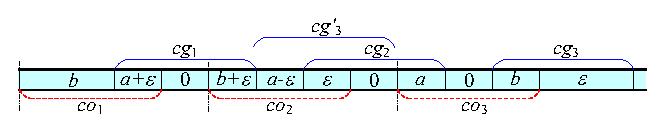
\includegraphics[width=0.48\textwidth]{rsu_example2p3.eps}}
\caption{An instance of the RDP problem where performance ratio of Greedy2P3 approaches 2/3.}
\label{fig_rsu_example2p3}
\end{figure}


\begin{equation}
\label{eq_greedy2p3_2}
\begin{array}{rl}
\beta_\text{G2P3}&{=}\frac{B(cg_1){+}B(cg_2){+}B(cg_3)}{B(co_1){+}B(co_2){+}B(co_3)}{=}\frac{2(a{+}b){+}3\varepsilon}{3(a{+}b){+}\varepsilon}
\mathop{=}\limits^{\varepsilon{\rightarrow}0^+}2/3\\
\end{array}
\end{equation}

For any $n{=}3*i$ ($i$ is an integer), we assume a road line consists of $i$ isolated road segments all identical to the example road line in Fig.\ref{fig_rsu_example2p3}. Then for this road line, it is easy to notice that the greedy strips and the optimal strips must forms $i$ strip groups identical to the strip group in Fig.\ref{fig_rsu_example2p3}. The performance ratio of Greedy2P3 on this problem instance will be 2/3.

Combining Eq.(\ref{eq_greedy2p3_1}) and Eq.(\ref{eq_greedy2p3_2}), we obtain that the performance ratio of Greedy2P3 on any RDP instance is at least 2/3, and this value is reachable. Hence, Greedy2P3's approximation ratio $\alpha_\text{G2P3}$ is at least 2/3, and it is tight for $n{=}3{*}i$.
\end{IEEEproof}

\textbf{Comment:}Although the approximation ratio is not very high, simulation results show that Greedy2P3 usually return quasi-optimal solutions with profit usually more than 98\% of optimal solutions.

Combining Theorem \ref{lemma_greedy_approx_ratio} and Lemma \ref{lemma_greedybetter}, we can obtain Theorem \ref{lemma_Greedy2P3E_approx_ratio} directly.

\begin{theorem}
\label{lemma_Greedy2P3E_approx_ratio}
The approximation ratio of Greedy2P3E for one-dimensional RDP problem with $n$ identical RSUs is at least $\text{max}\{1{-}(\frac{n{-}1}{n})^n,2/3\}{=}\left\{\substack{1{-}(\frac{n{-}1}{n})^n, \hspace{1mm}\text{If}\hspace{1mm}n{\leq}5;\\2/3,\hspace{1mm}\text{If}\hspace{1mm}n{\geq}6;}\right.$.
\end{theorem}

\section{Performance Evaluation}
\label{sec_sim}
\subsection{Performance Metrics}

In order to verify the analysis results and evaluate the performance of the proposed algorithms, we conduct numerical simulations using Matlab 2015b on a computer with Win7-bit64, 2GHz CPU, and 4GB Memory. Three performance metrics are used: \textbf{Solution profit, Run time(s), and Try number}. The solution profit metric represents the profit of a solution. The run time metric measures the average time used to solve a RDP problem instance. The metric of try number measures the number of candidate solutions checked by an algorithm, which is used to evaluate the effectiveness of optimal algorithms in reducing search space. Here we compare our optimal algorithm OptGreDyn with two other optimal algorithms named as OptAll and OptDynLim. OptDynLimit utilizes the dynamic limiting technique introduced in Section \ref{sec_dynlim}. OptAll uses the exhaustive search approach.

Quite a few works have been conducted in the literature, where greedy based approach is widely used. These greedy algorithms are adapted to variants of the RDP problem with particular restrictions and assumptions. Most works assume that RSUs can only be deployed at road intersections \cite{Trullols2010} or middle roads\cite{Kafsi2008}. Hence, for comparative evaluation on our approximate algorithms Greedy2P3 and Greedy2P3E, we add two typical previous algorithms into our simulation experiments, marked respectively as GreedyMiddle and BEP. GreedyMiddle is a representation of existing greedy based algorithms, which determines RSUs' positions greedily one by one, but only middle points of segments are considered as valid candidate positions. The BEP algorithm represents the Balloon Expansion Heuristic(BEH) algorithm proposed in \cite{Aslam2012}, which is adapted to our one-dimensional problem here. In BEP, only segment ends are valid candidate positions for RSUs. BEP works as follows. At first, a RSU is assumed at each candidate positions, then this RSUs expand their coverage radius from zero to $d/2$ gradually. In this process, RSUs with overlapped coverages are replaced with one representative RSU selected from the RSUs. At last, the best $n$ RSUs in term of profit form the final solution.

   BEP first assumes that  at The idea underlie BEP is very distinctive, so it is also included here.

\subsection{Simulation Setup}
The profit density functions of the segments make difference only in the construction of $X_\text{cand,c}(n,d)$ and the profit of the strips in $X_\text{cand,c}(n,d)$. Later operations in an algorithm need only work on $X_\text{cand,c}(n,d)$, whereas the profit density functions are not needed any longer. The construction of $X_\text{cand}$ is straightforward, so main results in our work need to be verified are on one-dimensional RDP problem with multiple identical RSUs. Hence, without deceasing the credibility of our experiments, we only perform simulations on cases where roads have piecewise constant functions.

Main parameters used for simulating our RDP problem with identical RSUs include (1) number of RSUs $n$, (2) strip length $d$, i.e., diameter of the circular coverage of the RSUs, (3) length of the whole road line $L_\text{road}$, (4) average length of a road segment $L_\text{seg}$, and (5) the upper limit $w_\text{max}$ of the profit density function value of a road segment. A set of particular values for these parameters is called a simulation configuration. For each configuration, 100 problem instances are generated and then treated using the tested algorithms in turn. In each problem instance, $\text{round}(\frac{L_\text{road}}{L_\text{seg}}){-}1$ points are generated randomly in range $(0,L_\text{road})$ following uniform distribution. These points are used as segment end points, which divide the whole road line into $L{=}\text{round}(\frac{L_\text{road}}{L_\text{seg}})$ segments. These segments all have constant profit density functions, where the constants take integer values randomly from [0,$w_\text{max}$] following uniform distribution. Data for the performance metrics are collected and averaged to obtain the final results for the configuration. Hence, each point in the figures in later subsections showing simulation results corresponds to 100 simulations. The 95\% confidence intervals of the performance metrics are also obtained.

The effect of a parameter on an algorithm's performance is usually tested by performing a simulation set consisting of several simulation configurations. In these configurations, only the parameter to be tested take different values, whereas the other parameters usually take default values. In our simulation, the parameters' default values are $n{=}5$, $d{=}4$, $L_\text{road}{=}200$, $L_\text{seg}{=}3$, and $w_\text{max}{=}10$.

\subsection{Size of Candidate Strip Sets}
\begin{figure}[htbp]
\centering{
\begin{minipage}[c]{0.23\textwidth}
\centering{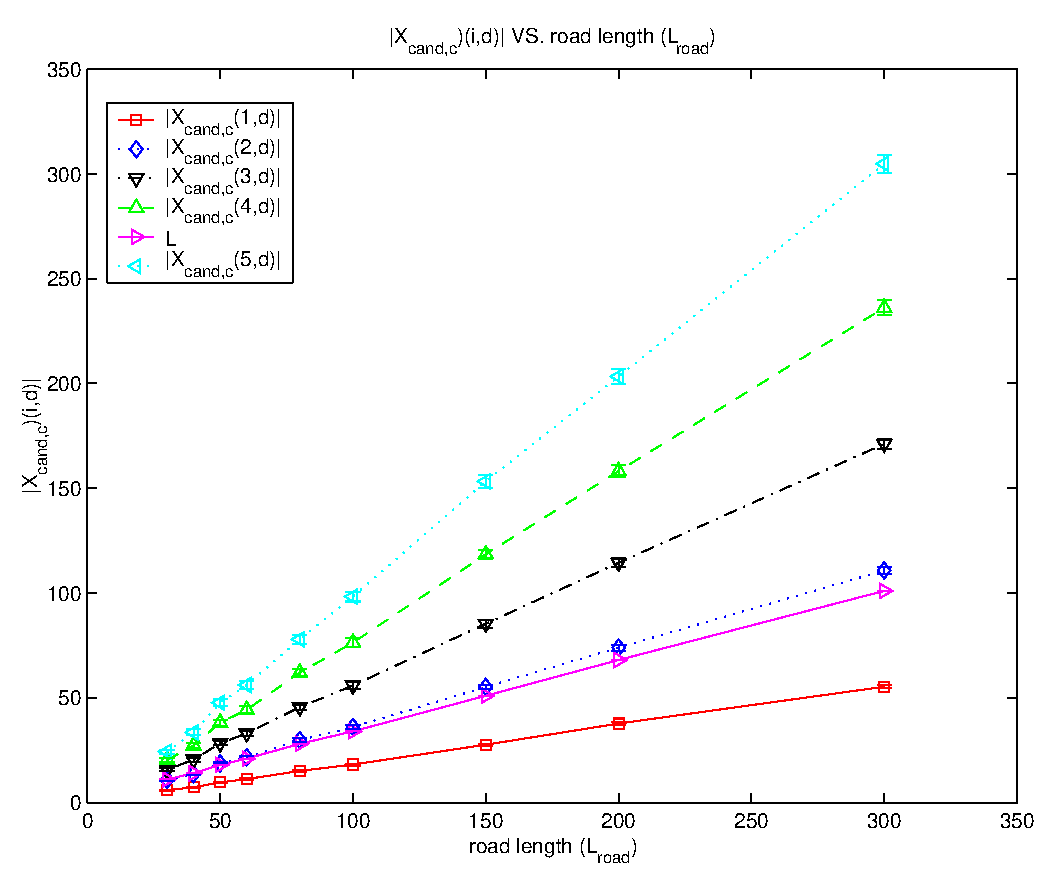
\includegraphics[width=\textwidth]{sim_candnum_road.eps}}
\parbox{\linewidth}{\centering\small (a)}
\end{minipage}%
\hspace{0.01\textwidth}%
\begin{minipage}[c]{0.23\textwidth}
\centering{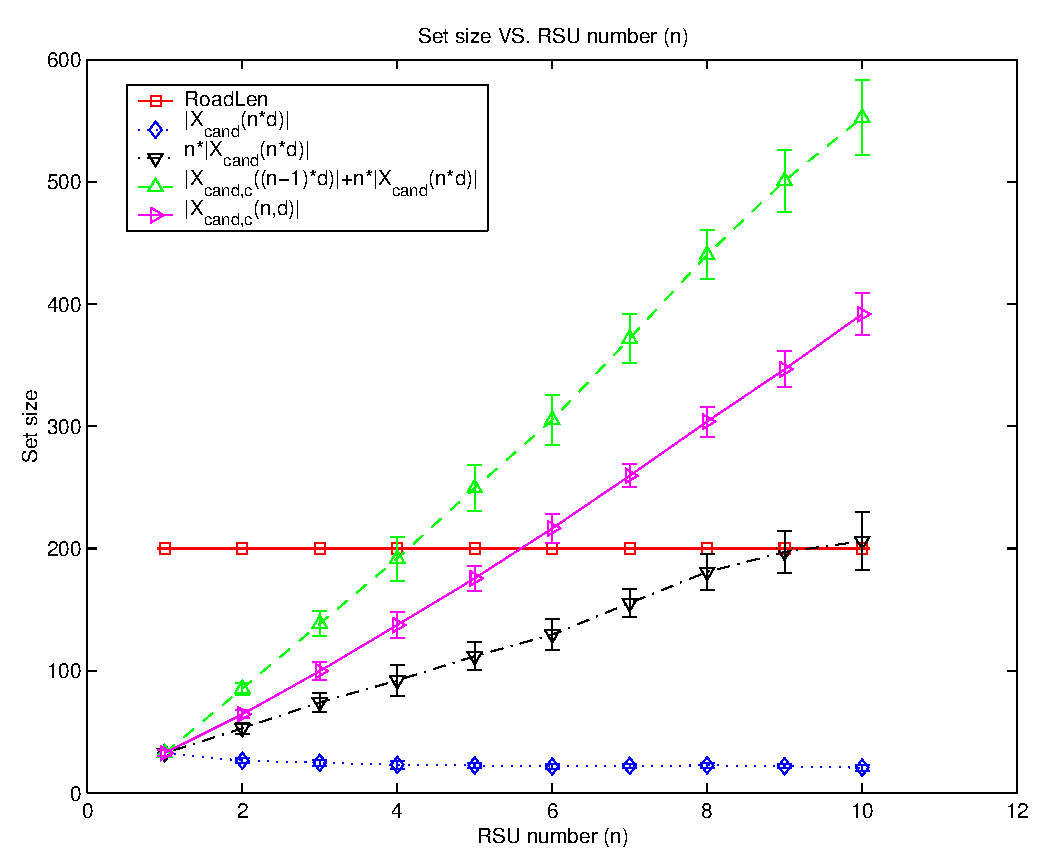
\includegraphics[width=\textwidth]{sim_candnum_rsunum.eps}}
\parbox{\linewidth}{\centering\small (b)}
\end{minipage}
}
\caption{The effects of $L_\text{road}$ and $n$ on the size of candidate strip sets.}
\label{fig_sim_cannum}
\end{figure}

It is obvious that $|X_\text{cand,c}(n,d)|$ has a great effect on the execution time of the algorithms. We first inspect the relation between $|X_\text{cand,c}(n,d)|$ and the parameters. We only provide the results for $L_\text{road}$ and $n$ in Fig.\ref{fig_sim_cannum}. The results for other parameters show no new insights and are thus omitted for space limitation. Fig.\ref{fig_sim_cannum}(a) shows the effect of $L_\text{road}$, where it takes values from the list $\{30,40,50,60,80,100,150,200,300\}$. Fig.\ref{fig_sim_cannum}(b) shows the effect of $n$, where it takes values from 1 to 10. To get better understandings, some additional information are also collected. Fig.\ref{fig_sim_cannum}(a) also show the results of $|X_\text{cand,c}(i,d)|$, $i{\in}\{1,\ldots,n\}$. In Fig.\ref{fig_sim_cannum}(b), other data as indicated by the legends are shown. The results show that, $|X_\text{cand,c}(i,d)|$ increase both linearly along $L$ and $n$, which consists with the rough analysis result of $|X_\text{cand,c}(n,d)|{=}\mathcal{O}(n{*}L)$ in Section \ref{sec_analysis_identical}.

\subsection{Simulation Results}
The results of the performance metrics in the previous experiment with different $L_\text{road}$ are shown in Fig.\ref{fig_sim_roadlen}. Fig.\ref{fig_sim_roadlen}(a) shows that, profits of the solutions obtained by OptGreDyn, OptDynLim are both identical to that of OptAll, which confirm the optimality of OptGreDyn and OptDynLim. In the simulated cases, our two approximate algorithms Greedy2P3 and Greedy2P3E both return quasi-optimal solutions, with profit more than 98\% and 99\% of optimal solutions. Contrastively, GreedyMiddle and BEP are much less efficient. When $L_\text{road}{=}30$, profits of their solutions are both less than 80\% of optimal solutions, and GreedyMiddle solutions are slightly better than those of BEP. As $L_\text{road}$ increases,
solutions of GreedyMiddle approach optimal solutions gradually, whereas the differences between optimal solutions and those of BEP show no distinctive change. Results on run time metric are shown in Fig.\ref{fig_sim_roadlen}(b). As run time of OptAll increases to sharply, we omit the tests on OptAll when $L_\text{road}{\geq}60$. To show the results on the run time metric of other algorithms more clearly, we provide a new view in Fig.\ref{fig_sim_roadlen}(c), where the results of OptAll is removed. Compared with OptDynLim, OptGreDyn saves run time more than 50\%. Compared with OptGreDyn, Greedy2P3, Greedy2P3E, BEP save runtime by more than 40\%. Among the tested algorithms, GreedyMiddle is the most time efficient one, whose run time is only about 30\% of OptGreDyn. Fig.\ref{fig_sim_roadlen}(d) shows the results on try number metric. The results show that, compared with OptDynLim, OptGreDyn reduces search space size by more than 75\%. As a conclusion, OptGreDyn is an efficient optimal algorithm, and Greedy2P3 and Greedy2P3E are more preferable than BEP and GreedyMiddle when considering both solution profit and run time.

\begin{figure}[htbp]
\centering{
\begin{minipage}[c]{0.23\textwidth}
\centering{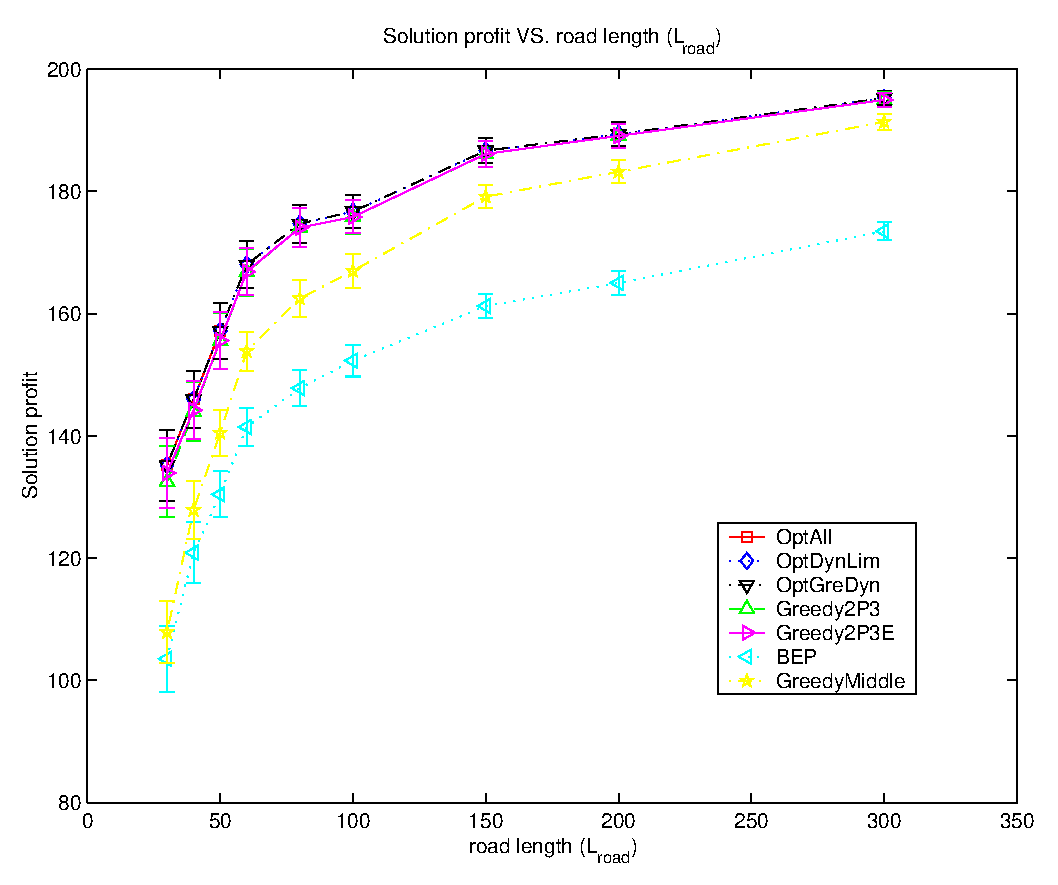
\includegraphics[width=\textwidth]{sim_roadlen_profit.eps}}
\parbox{\linewidth}{\centering\small (a)}
\end{minipage}%
\hspace{0.01\textwidth}%
\begin{minipage}[c]{0.23\textwidth}\centering{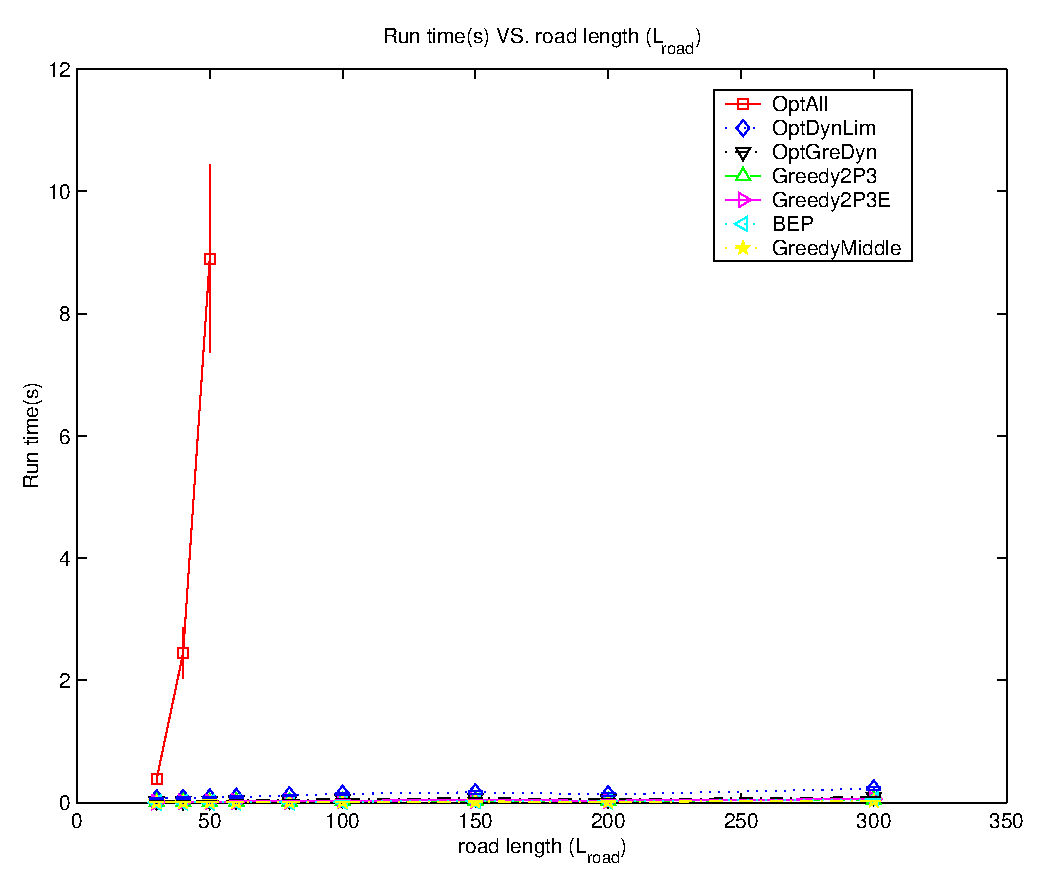
\includegraphics[width=\textwidth]{sim_roadlen_time.eps}}
\parbox{\linewidth}{\centering\small (b)}
\end{minipage}
}
\\
\centering{
\begin{minipage}[c]{0.23\textwidth}
\centering{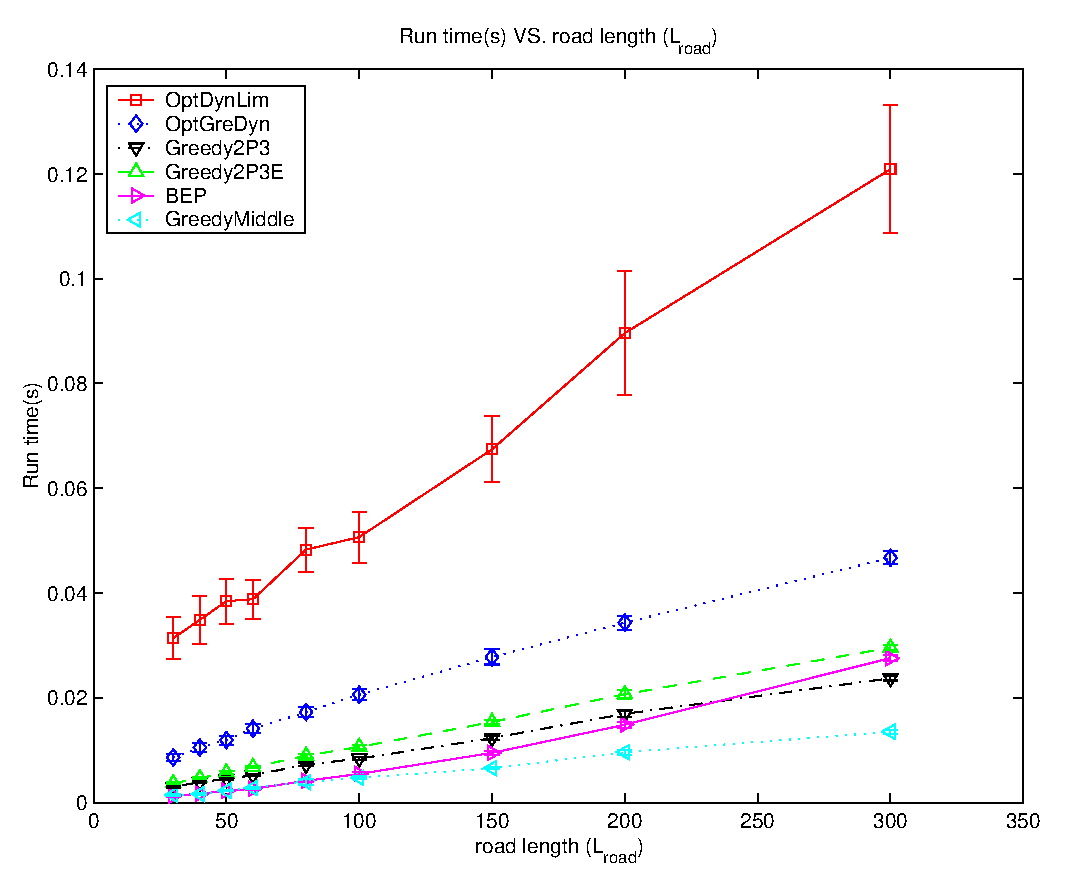
\includegraphics[width=\textwidth]{sim_roadlen_timezoom.eps}}
\parbox{\linewidth}{\centering\small (c)}
\end{minipage}
\hspace{0.01\textwidth}%
\begin{minipage}[c]{0.23\textwidth}
\centering{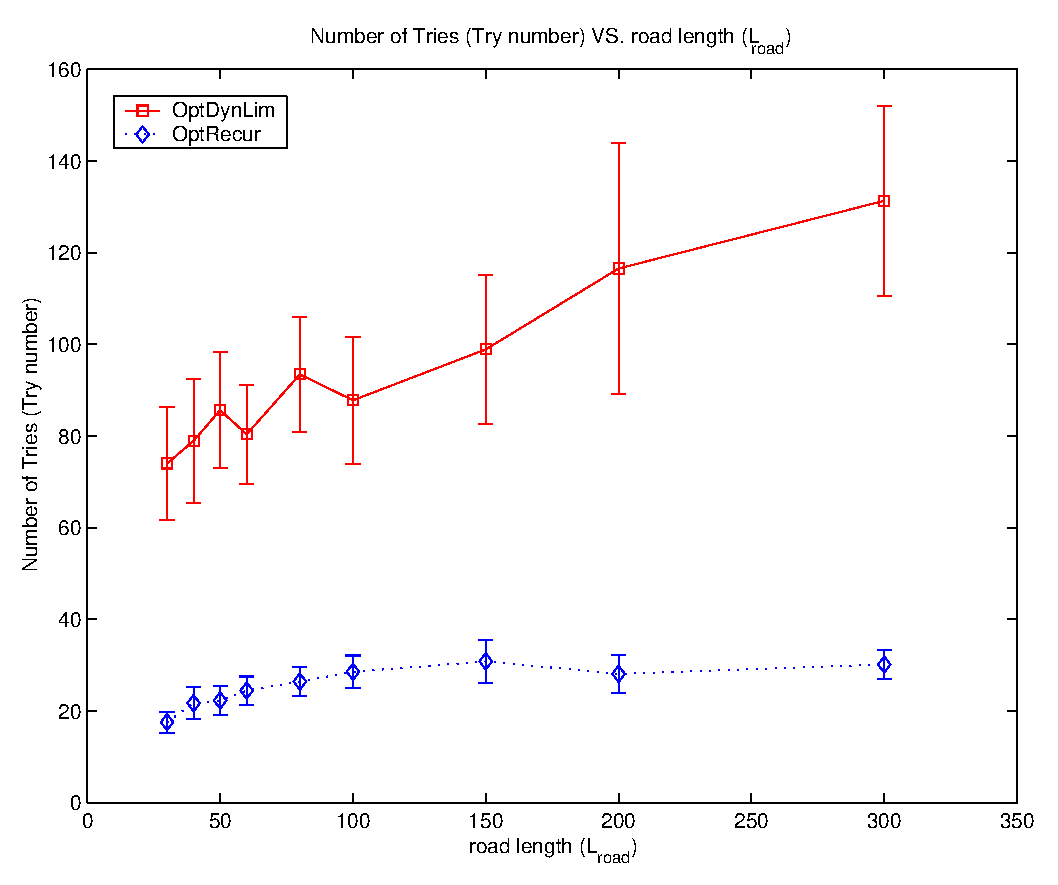
\includegraphics[width=\textwidth]{sim_roadlen_trynum.eps}}
\parbox{\linewidth}{\centering\small (d)}
\end{minipage}
}
\caption{The effects of $L_\text{road}$ on algorithms' performances, (a)solution profit, (b)run time, (c)run time of the algorithms without OptAll, (d)try number}
\label{fig_sim_roadlen}
\end{figure}

We have conduct other experiments for inspecting the effects of all other main parameters ($n$, $d$, $L_\text{seg}$, $W_\text{max}$). In these experiments, OptAll is omitted since that the optimality of OptGreDyn and OptDynLim have been verified in the previous simulations. Simulation results all demonstrate that Greedy2P3 and Greedy2P3E usually return quasi-optimal solutions with profit more than 98\% of optimal ones. Greedy2P3 and Greedy2P3E are preferable than BEP and GreedyMiddle. For space limitation, we only provide the results corresponding to parameter $n$ in Fig.\ref{fig_sim_rsunum_profit_time}, where $n$ takes values from 2 to 10 with step size 1. The solution profit results in Fig.\ref{fig_sim_rsunum_profit_time}(a) show that Greedy2P3 and Greedy2P3E both return nearly optimal solutions with profit more than 99\% of optimal ones. GreedyMiddle's solutions are less optimal with profit less than 93\% of optimal ones. Furthermore, as $n$ increases, the difference between GreedyMiddle's solution profit and that of the optimal solutions increases gradually. In the test cases, solutions of BEP are always the worst one. Fig.\ref{fig_sim_rsunum_profit_time}(b) shows the run time metric of the algorithms. As $n$ increases, run time of both OptGreDyn and OptDynLim increases quickly, but the increasing speed of OptGreDyn is obviously slower than that of OptDynLim. Contrastively, run time of the approximate algorithms are trivial. To show the results for the approximate algorithms more clearly, a zoomed view is provided in Fig.\ref{fig_sim_rsunum_profit_time}(b). Run time of Greedy2P3, Greedy2P3E, and GreedyMiddle all increase near linearly as $n$ increases, which is reasonable considering how they work. BEP's run time does not vary much as $n$ increases, which is reasonable since that its operation procedure doesn't rely on $n$ heavily. The curves for the run time metric and the try number metric show similar trends, so the figure corresponding to the try number metric is omitted here.

\begin{figure}[htbp]
\centering{
\begin{minipage}[c]{0.23\textwidth}
\centering{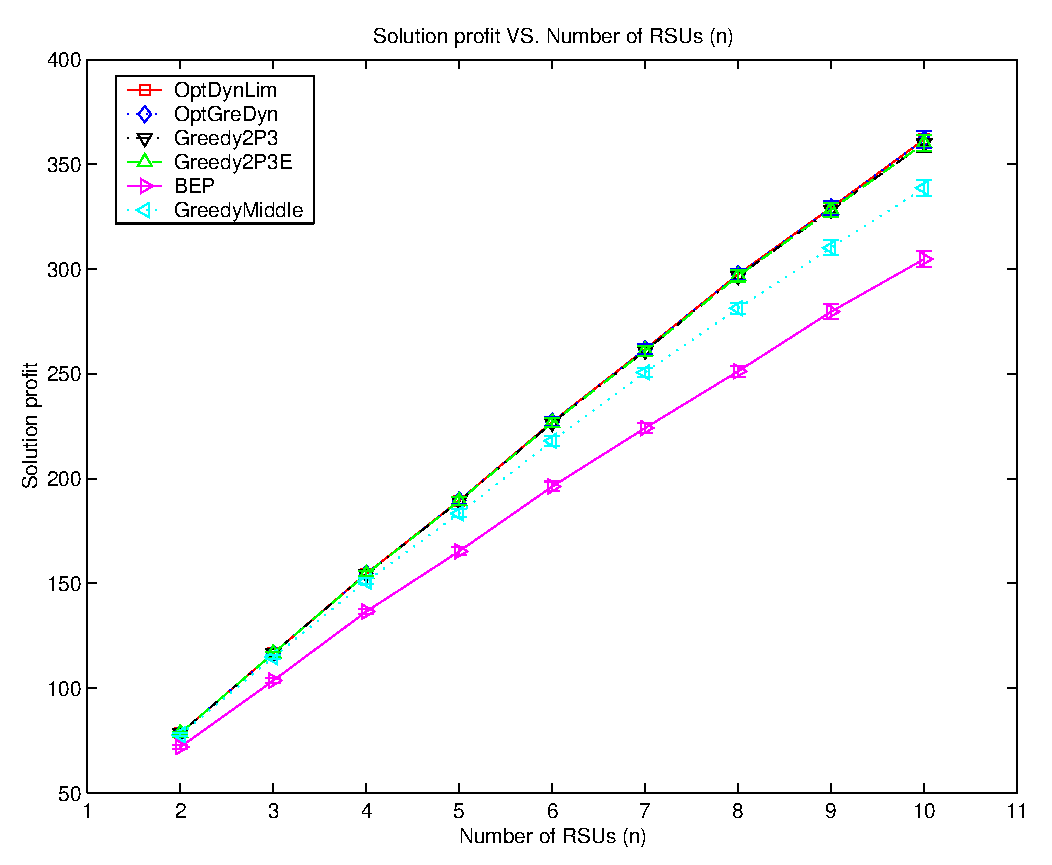
\includegraphics[width=\textwidth]{sim_rsunum_profit.eps}}
\parbox{\linewidth}{\centering\small (a)}
\end{minipage}%
\hspace{0.01\textwidth}%
\begin{minipage}[c]{0.23\textwidth}
\centering{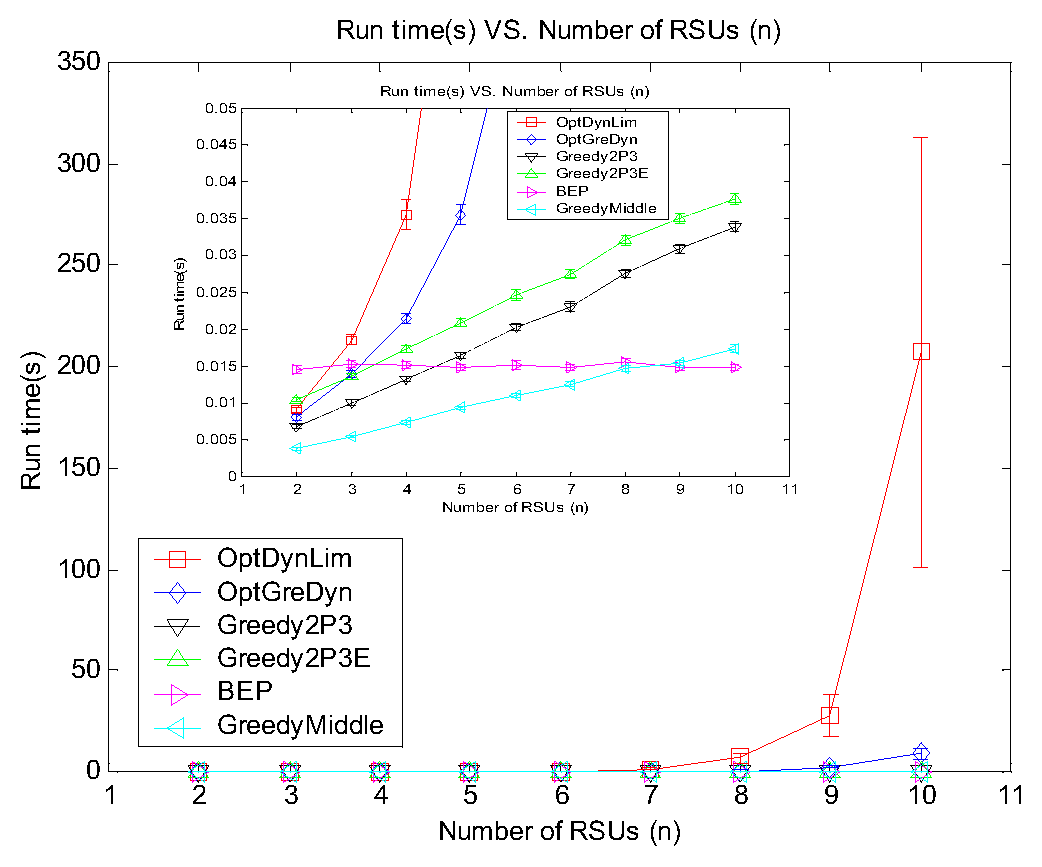
\includegraphics[width=\textwidth]{sim_rsunum_time.eps}}
\parbox{\linewidth}{\centering\small (b)}
\end{minipage}}
\caption{The effect of $n$ on performance, (a) solution profit, (b) run time.}
\label{fig_sim_rsunum_profit_time}
\end{figure}

% An example of a floating figure using the graphicx package.
% Note that \label must occur AFTER (or within) \caption.
% For figures, \caption should occur after the \includegraphics.
% Note that IEEEtran v1.7 and later has special internal code that
% is designed to preserve the operation of \label within \caption
% even when the captionsoff option is in effect. However, because
% of issues like this, it may be the safest practice to put all your
% \label just after \caption rather than within \caption{}.
%
% Reminder: the "draftcls" or "draftclsnofoot", not "draft", class
% option should be used if it is desired that the figures are to be
% displayed while in draft mode.
%
%\begin{figure}[!t]
%\centering
%\includegraphics[width=2.5in]{myfigure}
% where an .eps filename suffix will be assumed under latex,
% and a .pdf suffix will be assumed for pdflatex; or what has been declared
% via \DeclareGraphicsExtensions.
%\caption{Simulation Results.}
%\label{fig_sim}
%\end{figure}

% Note that IEEE typically puts floats only at the top, even when this
% results in a large percentage of a column being occupied by floats.


% An example of a double column floating figure using two subfigures.
% (The subfig.sty package must be loaded for this to work.)
% The subfigure \label commands are set within each subfloat command,
% and the \label for the overall figure must come after \caption.
% \hfil is used as a separator to get equal spacing.
% Watch out that the combined width of all the subfigures on a
% line do not exceed the text width or a line break will occur.
%
%\begin{figure*}[!t]
%\centering
%\subfloat[Case I]{\includegraphics[width=2.5in]{box}%
%\label{fig_first_case}}
%\hfil
%\subfloat[Case II]{\includegraphics[width=2.5in]{box}%
%\label{fig_second_case}}
%\caption{Simulation results.}
%\label{fig_sim}
%\end{figure*}
%
% Note that often IEEE papers with subfigures do not employ subfigure
% captions (using the optional argument to \subfloat[]), but instead will
% reference/describe all of them (a), (b), etc., within the main caption.


% An example of a floating table. Note that, for IEEE style tables, the
% \caption command should come BEFORE the table. Table text will default to
% \footnotesize as IEEE normally uses this smaller font for tables.
% The \label must come after \caption as always.
%
%\begin{table}[!t]
%% increase table row spacing, adjust to taste
%\renewcommand{\arraystretch}{1.3}
% if using array.sty, it might be a good idea to tweak the value of
% \extrarowheight as needed to properly center the text within the cells
%\caption{An Example of a Table}
%\label{table_example}
%\centering
%% Some packages, such as MDW tools, offer better commands for making tables
%% than the plain LaTeX2e tabular which is used here.
%\begin{tabular}{|c||c|}
%\hline
%One & Two\\
%\hline
%Three & Four\\
%\hline
%\end{tabular}
%\end{table}


% Note that IEEE does not put floats in the very first column - or typically
% anywhere on the first page for that matter. Also, in-text middle ("here")
% positioning is not used. Most IEEE journals use top floats exclusively.
% Note that, LaTeX2e, unlike IEEE journals, places footnotes above bottom
% floats. This can be corrected via the \fnbelowfloat command of the
% stfloats package.

\section{Conclusions}
\label{sec_conclusion}
In this paper, we focus on the one-dimensional RDP problem with our new model. We firstly analyze the properties of optimal solutions of the RDP problem. Then, suspecting that the one-dimensional RDP problem with $n$ RSUs of different radii is intractable, we propose two greedy-based algorithms (named as Greedy2P3 and Greedy2P3E) and show that Greedy2P3E's approximation ratio is at least $1{-}(\frac{n{-}1}{n})^2$. And next, for the one-dimensional RDP problem with $n$ RSUs of identical radii, we found that it can be transformed to a problem being a subset of the well-known maximum coverage problem, which is NP-hard. By exploiting the properties of optimal solutions of the original problem, we propose an optimal algorithm based on greedy idea and dynamic programming, so it is abbreviated as OptGreDyn. At last, we proved that, if applied to the one-dimensional RDP problem with $n$ RSUs of identical radii, the approximation ratios of Greedy2P3 and Greedy2P3E are at least 2/3. Furthermore, Greedy2P3's approximation ratio of 2/3 is tight when $n{=}3{*}i$, here $i$ is any positive integer. Numerical simulations validate the correctness of the analyses results. Simulation results verify the optimality of OptGreDyn, meanwhile show that Greedy2P3 and Greedy2P3E usually return near-optimal solutions with more than 99\% of optimal solutions, and they are preferable than existing approximate algorithms.

Several open issues about the new RDP problem require further research efforts, such as problem complexity analysis to one-dimensional RDP problem and two RDP problem, tighter approximation ratio of better greedy algorithms including our Greedy2P3E. Efforts on better approximate algorithms for the new RDP problem with multiple heterogenous RSUs are also needed.

% if have a single appendix:
%\appendix[Proof of the Zonklar Equations]
% or
%\appendix  % for no appendix heading
% do not use \section anymore after \appendix, only \section*
% is possibly needed

% use appendices with more than one appendix
% then use \section to start each appendix
% you must declare a \section before using any
% \subsection or using \label (\appendices by itself
% starts a section numbered zero.)
%

\appendices
\section{Proof Preparations of of Theorem \ref{lemma_greedy_approx_ratio}}
\label{secAppGreedy}
The whole process for proving the approximation ratio of Greedy2P3 can be roughly expressed in 5 steps as follows.
\begin{enumerate}[\textbf{Step}1:]
\item We totally identify 15 cell styles, and determine whether they are stable, unstable, invalid. (Refer to Appendix \ref{secApp_greedy_cs}).
\item Based on the properties of the cell styles, and using the fact that an unstable cell must join a group by connecting to stable cells through paths, we identify 8 group styles (Refer to Appendix \ref{secApp_greedy_gs}).
\item We make all unbalanced groups become balanced by using logic rearrangement operations. We identify 6 logic group styles (Refer to Appendix \ref{secApp_greedy_lgs}).
\item For each logic group style, we prove its performance ratio(Refer to Appendix \ref{secApp_greedy_lgspr}).
\item We prove the approximation ratio of the Greedy2P3 algorithm by combining performance ratios of the logic group styles, and show that it is tight by providing some problem instances which can approach this approximation ratio.
\end{enumerate}

In this section, we will provide detailed process for the first four steps in the following four subsections, respectively.

\subsection{Cell Styles}
\label{secApp_greedy_cs}
Restricted to at most 3 strips, there are totaly 15 cell styles, as shown in Fig.\ref{fig_rsu_cellstyle}. In this figure, each sub-figure represents a cell style. Belts with lighter blue background represent road lines. Red brackets under road line represent optimal strips, whereas blue brackets over road line represent greedy strips. An arrow from strip $a$ to strip $b$ represents that $B(b){\geq}B(a)$. The cell style in Fig.\ref{fig_rsu_cellstyle}(a) is denoted as $CS_a$, other cell styles are denoted similarly. Some cell styles looks similar, such as $CS_{d1}$, $CS_{d2}$, $CS_{d3}$, $CS_{d4}$, thus we can also regard them as sub-styles of a virtual super style $CS_d$.

\begin{figure*}[ht]
\centering{
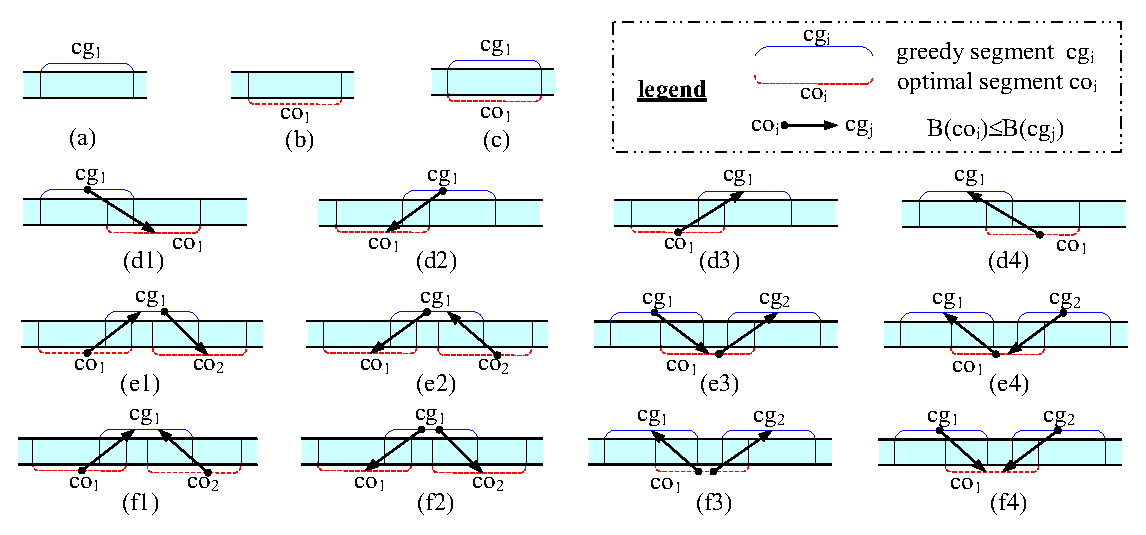
\includegraphics[width=0.9\textwidth]{rsu_cellstyle.eps}
}
\caption{Cell styles.}
\label{fig_rsu_cellstyle}
\end{figure*}

For cell styles, we obtain properties in terms of stable, unstable, and invalid. Main properties are as follows.

\begin{property}
\label{lemma_cs_ab}
If $B(cg_1){\neq}B(co_1)$, then cell styles $CS_a$ and $CS_b$ can not co-exist with each other.
\end{property}

\begin{IEEEproof}
We prove it by contraction. For any greedy solution $S_g$ and optimal solution $S_o$, we assume that some cells of style $CS_a$ and $CS_b$ co-exists. Then, for any greedy strip $cg_1$ of style $CS_a$ and any optimal strip $co_1$ of style $CS_b$, we have the following two cases.

\begin{itemize}
\item{Case: $B(cg_1){>}B(co_1)$}
\end{itemize}

In this case, by replacing $co_1$ in $S_o$ with $cg_1$, we can obtain a new solution $S_{o2}$. It is obvious that $B(S_{o2}){>}B(S_o)$, so $S_o$ must not be an optimal solution. This contradicts with the fact that solution $S_o$ is optimal.

\begin{itemize}
\item{Case: $B(cg_1){<}B(co_1)$}
\end{itemize}

In this case, $cg_1$ will not be selected by Greedy2P3 since that $cg_1$ is not the best free strip because that $B(cg_1){<}B(co_1)$. This contradicts with the fact that $cg_1$ is a greedy strip.

Combining the above results, we complete the proof.
\end{IEEEproof}

\begin{property}
\label{lemma_cs_a}
For the two cell styles $CS_a$ and $CS_b$, If only $CS_a$ exists, then any optimal strips must have profit not smaller than any of the $CS_a$ strips. If only $CS_b$ exists, then any greedy strips must have profit not smaller than any of the $CS_b$ strips.
\end{property}

\begin{IEEEproof}
We only provide the proof for the case that only $CS_a$ exists. The proof for the other case can be completed similarly.
We prove it by contradiction. If only $CS_a$ exists, we assume that there is an optimal strip $os_1$ that satisfies $B(os_1){<}B(gs_1)$. In this case, we can replace $os_1$ in the optimal solution(denoted as $S_1$) with strip $gs_1$, we thus obtain a solution $S_2$ with $B(S_2){>}B(S_1)$, which contradicts with the fact that solution $S_1$ is optimal.
\end{IEEEproof}

\begin{property}
\label{lemma_cs_d1}
If $B(cg_1){\neq}B(co_1)$, then cell styles $CS_{d1}$,$CS_{d2}$,$CS_{d3}$ and $CS_{d4}$ are unstable.
\end{property}

\begin{IEEEproof}
Here we only provide the proof for cell style $CS_{d1}$. The results for the other three styles can be proved similarly.

As shown in style $CS_{d1}$ in Fig.\ref{fig_rsu_cellstyle}, we have $B(cg_1){\leq}B(co_1)$. We will prove it with the help of Fig.\ref{fig_rsu_extension}. If $B(cg_1){\neq}B(co_1)$, then we have $B(cg_1){<}B(co_1)$. Since that Greedy2P3 will select the maximum free strip at each time, the fact of $B(cg_1){<}B(co_1)$ implies that strip $co_1$ must be connected with another greedy coverage, say $cg_2$, as shown in Fig \ref{fig_rsu_extension}(a), which prevents Greedy2P3 from selecting $co_1$. Otherwise, $cg_1$ will not be the maximum free strip at the time to select $cg_1$. We step further, if $B(co_1){<}B(cg_2)$, then the strip set $\{cg_1,co_1,cg_2\}$ should also be connected to other strips. Otherwise, $co_1$ will not be an optimal strip since that replacing $co_1$ with $cg_2$ will obtain a better solution. Hence, there must be another optimal strip $co_2$ to which $cg_2$ directly connects. Such analysis process can continue until it meets one of the two cases: (1) $B(cg_i){\geq}B(co_{i})$, (2)$B(cg_{i{+}1}){=}B(co_{i})$.
\begin{itemize}
\item{Case $B(cg_i){\geq}B(co_{i})$:}
\end{itemize}
In this case, the strip set $\{co_{i{-}1},cg_i,co_{i}\}$ forms an instance of cell style $CS_{f1}$, which is stable as shown in Property \ref{lemma_cs_f1}.

\begin{itemize}
\item{Case $B(cg_{i{+}1)}{=}B(co_{i})$:}
\end{itemize}
In this case, the strip set $\{cg_{i{+}1},co_i\}$ forms an instance of cell style $CS_{d2}$ or $CS_{d3}$. They all are stable when $B(cg_{i{+}1)}{=}B(co_{i})$.

As a conclusion, cell style $CS_{d1}$ is unstable when $B(cg_1){\neq}B(co_1)$. Cells of style $CS_{d1}$ can only exist by connecting to other stable cells. The property follows.
\end{IEEEproof}

\begin{figure}[ht]
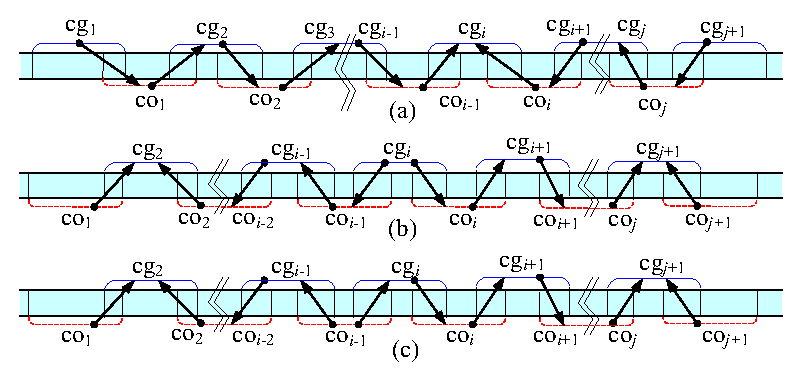
\includegraphics[width=0.48\textwidth]{rsu_extension.eps}
\caption{Extension of unstable cells.}
\label{fig_rsu_extension}
\end{figure}

The following two properties can be proved similarly.

\begin{property}
\label{lemma_cs_e1}
If $B(cg_1)$, $B(cg_2)$, $B(co_1)$, $B(co_2)$ are all different, then cell styles $CS_{e1}$,$CS_{e2}$,$CS_{e3}$ and $CS_{e4}$ are unstable.
\end{property}

\begin{property}
\label{lemma_cs_f1}
If $B(cg_1){<}B(co_1)$ or $B(cg_1){<}B(co_2)$, then sell style $CS_{f2}$ is unstable. If $B(co_1){<}B(cg_1)$ or $B(co_1){<}B(cg_2)$, then sell style $CS_{f3}$ is unstable.
\end{property}

Cell style $CS_{f4}$ has the following property.

\begin{property}
\label{lemma_cs_f4}
If $B(cg_1){<}B(co_1)$ and $B(cg_2){<}B(co_1)$, then cell style $CS_{f4}$ is invalid.
\end{property}

\begin{IEEEproof}
We prove it by contradiction. Without lost generality, we assume that Greedy2P3 selects $cg_1$ before $cg_2$. However, Greedy2P3 will actually not select $cg_1$ since that $cg_1$ is not the best free strip, as implied by the fact $B(co_1){>}B(cg_1)$. Thus there is a contradiction. The property follows.
\end{IEEEproof}

It is obvious that all other cell styles are stable. Furthermore, when the formulae represented by the arrows in these cell styles take equality, the cell styles are all stable. For example, if $B(cg_1){=}B(co_1)$, then all cell styles $CS_{di}$, $i{\in}\{1,2,3,4\}$, are stable. If $B(cg_1){=}B(co_2)$, then we can reverse the directions of the corresponding arrows in cell styles $CS_{e,1}$ and $CS_{e,2}$. These cell styles thus become cell styles $CS_{f1}$ and $CS_{f2}$, respectively. Similarly, if $B(cg_1){=}B(co_2)$, then cell styles $CS_{e,3}$ and $CS_{e,4}$ can be transformed to cell styles $CS_{f,3}$ and $CS_{f,4}$ by reversing the directions of the corresponding arrows.

\subsection{Group Styles}
\label{secApp_greedy_gs}
Unstable cells can only exist actually by connecting to stable cells directly or indirectly. So, for any unstable cell, there must be one or two paths that connect the unstable cell to stable ones. For example, in Fig.\ref{fig_rsu_extension}(a), the unstable cell $\{cg_1,co_1\}$ of style $CS_{d1}$ connects to stable cell $\{co_{i{-}1}, cg_i, co_i\}$ of style $CS_{f1}$ through a path. In fact, such paths are formed by unstable cells. Meanwhile, another unstable cell $\{co_{j},cg_j{+}1\}$ of style $CS_{d2}$ connects to the same stable cell at the right side. In Fig.\ref{fig_rsu_extension}(b), an unstable cell $\{co_{i{-}1},cg_i,co_i\}$ of style $CS_{f2}$ is connected to two stable cells of style $CS_{f1}$ (they are $\{co_1,cg_2,co_2\}$ and $\{co_j,cg_{j{+}1},co_{j{+}1}\}$) from the left side and right side, respectively. In Fig.\ref{fig_rsu_extension}(c), the paths connecting an unstable cell $\{cg_{i{-}1}, co_{i{-}1}, cg_{i}\}$ of style $CS_{f3}$ to two stable cells of style $CS_{f1}$ (they are $\{co_1,cg_2,co_2\}$ and $\{co_j,cg_{j{+}1},co_{j{+}1}\}$) are shown.

Thus, through paths, cells are grouped into strip groups. There are totally eight group styles, as shown in Fig.\ref{fig_rsu_group}. The group style in Fig.\ref{fig_rsu_group}(a) is denoted as $GS_a$. Other group styles are denoted similarly. For expression brevity, the latter five group styles from $GS_d$ to $GS_h$ are illustrated using abbreviated symbols, where red bars in the lower layers represent optimal strips, blue bars in the upper layers represent greedy strips. A bi-directional arrow represents an arrow with either direction. A line without arrow ends represents the only case that the two strips have exactly the same profit. A part marked with three continuous small circles means that the part can happen zero or more times.

\begin{figure}[ht]
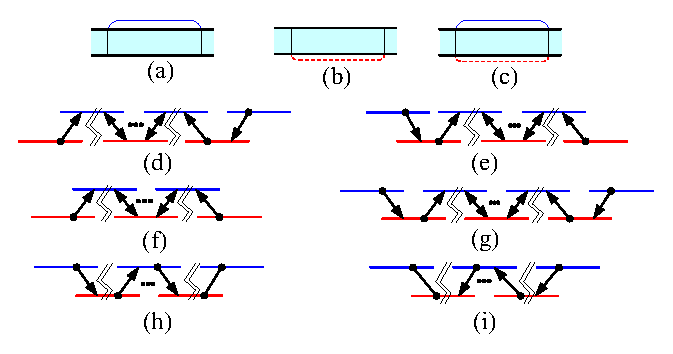
\includegraphics[width=0.48\textwidth]{rsu_groupstyle.eps}
\caption{Group styles.}
\label{fig_rsu_group}
\end{figure}

Group styles are abstract representations of many strip groups that can actually exist. For example, group style $GS_c$ can represent groups formed by cell style $CS_c$, or groups formed by stable cells of styles $CS_{di}$ when $B(cg_1){=}B(co_1)$, $i{\in}\{1,2,3,4\}$. The group in Fig.\ref{fig_rsu_extension}(a) is an instance of group style $GS_g$. The groups in Fig.\ref{fig_rsu_extension}(b) and Fig.\ref{fig_rsu_extension}(c) are both instances of group style $GS_f$. As in the proof of Property \ref{lemma_cs_d1}, if $B(co_{i{-}1}){=}B(cg_{i})$, the strip set $\{cg_1,co_1,\cdots,cg_{i{-}1},co_{i{-}1},cg_{i}\}$ forms a group of style $GS_h$.

\subsection{Logic Group Styles}
\label{secApp_greedy_lgs}
To facilitate performance analysis, balanced groups are preferred. For unbalanced group styles of $GS_a$, $GS_b$, $GS_f$, $GS_g$, $GS_h$ and $GS_i$, we can make them become balanced by logically rearranging some strips among different unbalanced groups. In the logic rearrangement operation, we do not move strips physically, instead, we just logically regard the strips as a member of the other group where it is logically inserted. Hence, final balanced groups are called as logic groups. Logic groups are be categorized into totally five logic group styles as shown in Fig.\ref{fig_rsu_logicgroup}. These logic group styles are denoted as $LGS_a$, $LGS_b$, $LGS_c$, $LGS_d$, and $LGS_f$, respectively.

The whole process of making all unbalanced groups become balanced is called as \textbf{logic rearrangement process}. The whole process can be roughly described as three steps. This process is demonstrated in Fig.\ref{fig_rsu_logicrearrange}, where in group of styles $GS_g$, $GS_h$ and $GS_i$, the strips marked with pentagons are the strips to be split off.

\begin{enumerate}[\textbf{Step}1:]
\item Logically split off one greedy strip from each group of styles $GS_g$, $GS_h$, $GS_i$, and collect all these strips together with possible $GS_a$ strips into a set $S$. These groups are thus become balanced logic groups of style $LGS_d$, $LGS_e$, $LGS_f$, respectively.
\item For each group of style $GS_f$, we randomly select a strip from the set $S$ and logically connect it to the rightmost optimal strip in the group, thus we obtain logic groups of style $LGS_b$. .
\item If groups of style $GS_b$ exist, then some strips will be left in set $S$. In this case, the number of the strips must be identical to that of $GS_b$ groups. So we can match $GS_b$ groups and strips in $S$ into pairs. According to Property \ref{lemma_cs_ab}, in each pair, the greedy strip must have profit not smaller than that of the optimal strip. Thus, each pair will be a logic group of style $LGS_a$. If groups of style $GS_b$ do not exist, then set $S$ after Step2 must become empty.
\end{enumerate}

\begin{figure}[ht]
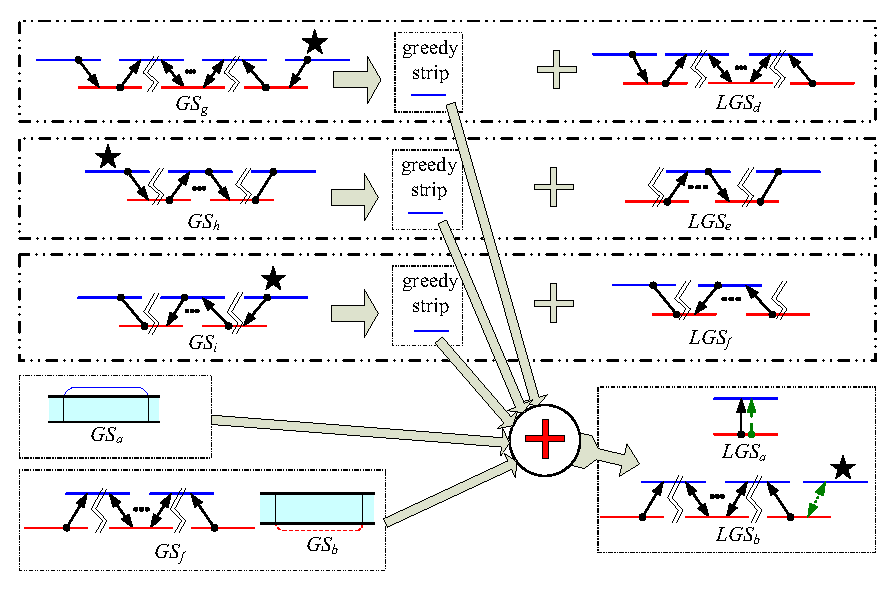
\includegraphics[width=0.48\textwidth]{rsu_logicrearrange.eps}
\caption{Logic rearrangement operation.}
\label{fig_rsu_logicrearrange}
\end{figure}

After the logic rearrangement process, all groups will be changed to logic groups, and they are all balanced groups.

\subsection{Performance Ratio of Greedy Algorithm on Logic Groups}
\label{secApp_greedy_lgspr}
In this section, we will analyze the performance ratios of Greedy2P3 respect to the logical groups. We use $\beta_\text{LGS}(i)$ to denote the performance ratio of Greedy2P3 on logic groups of style $LGS_i$, $i{\in}\{a,b,c,d,e,f\}$. It is obvious that $\beta_\text{LGS}(a){\geq}1$. The following lemmas show that $\beta_\text{LGS}(b){\geq}2/3$, $\beta_\text{LGS}(c){\geq}2/3$, $\beta_\text{LGS}(d){\geq}2/3$, $\beta_\text{LGS}(e){\geq}1$ and $\beta_\text{LGS}(f){\geq}1$.

\begin{lemma}
\label{lemma_lgsbcd_2p3}
For any logical group of style $LGS_b$,$LGS_c$ and $LGS_d$, there must be $\beta_\text{LGS}(b){\geq}2/3$, $\beta_\text{LGS}(c){\geq}2/3$ and $\beta_\text{LGS}(d){\geq}2/3$.
\end{lemma}

\begin{IEEEproof}
We only provide the proof for style $LGS_b$. The proof for the other two styles can be completed similarly.
Without loss of generality, we assume that the number of greedy strips and that of the optimal strips in a logic group of style $LGS_b$ is $m$. The detailed structure of the strip group is shown in Fig.\ref{fig_lgsb_cal2p3}, where the ends of the strips divides the road section into slices. For expression brevity, we roughly group the slices into $m{+}1$ sections, and each section contains 4 slices tagged with $a$, $b$, $c$ and $d$, respectively. The profit of slice $j$ in section $i$ is denoted as $x_{i,j}$. For example, $x_{2,b}$ represents the profit of the slice $b$ in section 2. This example is general enough to represent cases where all slices have different lengths. It can also represent cases where strips are adjacent. For example, $x_{i,b}{=}0$ can represent the case that two greedy strips are adjacent.

\begin{figure*}[htb]
\centering{\includegraphics[width=0.9\textwidth]{rsu_lgsb_cal2p3.eps}}
\caption{An example logical group of style $LGS_b$.}
\label{fig_lgsb_cal2p3}
\end{figure*}


The total profit of the greedy strips in the logical group, denoted as $B_\text{G}$, can be calculated as Eq.(\ref{eq_lgsb_1}). Here $G$ to represent the profit of the rightmost greedy strip, which is logically connected to the rightmost optimal strip.

\begin{equation}
\label{eq_lgsb_1}
B_\text{G}{=}G{+}\mathop{\sum}_{i{=}1}^{m{-}1}(x_{i,c}{+}x_{i,d}{+}x_{i{+}1,a})
\end{equation}

Similarly, the total profit of the optimal strips in the logical group, denoted as $B_\text{Opt}$, can be calculated as Eq.(\ref{eq_lgsb_2}).

\begin{equation}
\label{eq_lgsb_2}
B_\text{Opt}{=}\mathop{\sum}_{i{=}1}^{m}(x_{i,a}{+}x_{i,b}{+}x_{i,c})
\end{equation}

Simple mathematical transformations show that, the task of proving that $\beta_\text{LGS}(b){\geq}2/3$ is equivalent to prove Eq.(\ref{eq_lgsb_3}).

\begin{equation}
\label{eq_lgsb_3}
\begin{array}{rl}
2(x_{1,a}{+}x_{m,c}{+}\mathop{\sum}_{i{=}1}^{m}x_{i,b}){\leq}&\mathop{\sum}_{i{=}1}^{m{-}1}(x_{i,c}{+}x_{i{+}1,a})\\
&{+}3(G{+}\mathop{\sum}_{i{=}1}^{m{-}1}x_{i,d})
\end{array}
\end{equation}

No matter what directions are taken by the bi-directional arrows in the structural diagram of $LGS_b$, we have Eq.(\ref{eq_lgsb_4}), which can be checked easily. For example, when $i{=}2$, Eq.(\ref{eq_lgsb_4_1}) represents $x_{2,b}{\leq}(x_{2,d}{+}x_{3,a})$, which must be true. Otherwise, we have $B(cg'_2){\geq}x_{2,b}{+}x_{2,c}{>}x_{2,d}{+}x_{3,a}{+}x_{2,c}{=}B(cg_2)$. Thus, Greedy2P3 will select strip $cg'_2$ rather than $cg_2$. Since that all strips have the same length, strip $cg'_2$ must be able to cover the two slices of $x_{2,b}$ and $x_{2,c}$ completely.

\begin{subequations}
\label{eq_lgsb_4}
\begin{eqnarray}
x_{i,b}{\leq}x_{i,d}{+}x_{i{+}1,a},&2{\leq}i{\leq}m{-}1\label{eq_lgsb_4_1}\\
x_{i,b}{\leq}x_{i{-}1,c}{+}x_{i{-}1,d},&2{\leq}i{\leq}m{-}1\label{eq_lgsb_4_2}
\end{eqnarray}
\end{subequations}

According to the meaning of the leftmost arrow in Fig.\ref{fig_lgsb_cal2p3}, we have Eq.(\ref{eq_lgsb_5}).
\begin{equation}
\label{eq_lgsb_5}
x_{1,a}{+}x_{1,b}{\leq}x_{1,d}{+}x_{2,a}
\end{equation}

For the rightmost arrow, we must have Eq.(\ref{eq_lgsb_6}), otherwise strip $cg'_m$ will be selected by Greedy2P3 instead of the logically inserted strip with profit $G$.

\begin{equation}
\label{eq_lgsb_6}
x_{m,b}{+}x_{m,c}{\leq}G
\end{equation}

Furthermore, we must also have Eq.(\ref{eq_lgsb_7}), otherwise strip $cg'_0$ will be selected by Greedy2P3 instead of the logically inserted one with profit $G$.

\begin{equation}
\label{eq_lgsb_7}
x_{1,a}{+}x_{1,b}{\leq}G
\end{equation}

Accumulating both sides of the Equations in (\ref{eq_lgsb_4}), Eq.(\ref{eq_lgsb_5}), Eq.(\ref{eq_lgsb_7}), and 2 times of Eq.(\ref{eq_lgsb_6}), we obtain Eq.(\ref{eq_lgsb_8}).

\begin{equation}
\label{eq_lgsb_8}
\begin{array}{l}
2(x_{1,a}{+}x_{m,c}{+}\mathop{\sum}\limits_{i{=}1}^{m}x_{i,b}){\leq}(\mathop{\sum}\limits_{i{=}1}^{m{-}2}x_{i,c})
{+}(\mathop{\sum}\limits_{i{=}2}^{m}x_{i,a})\\
\hspace{0.1\textwidth}{+}x_{m{-}1,d}{+}2(\mathop{\sum}\limits_{i{=}2}^{m{-}1}x_{i,d}){+}3G
\end{array}
\end{equation}

Defining $f(x)$ as Eq.(\ref{eq_lgsb_9}), we have $f(x){\geq}0$ because that all variables in right side of $f(x)$ are non-negative.
\begin{equation}
\label{eq_lgsb_9}
f(x){\mathop{=}\limits^{\text{def}}}x_{m{-}1,c}{+}x_{m{-}1,d}{+}\mathop{\sum}\limits_{i{=}1}^{m{-}1}{x_{i,d}}
\end{equation}

Adding $f(x){\geq}0$ to Eq.(\ref{eq_lgsb_8}), we obtain Eq.(\ref{eq_lgsb_3}). The Lemma follows.
\end{IEEEproof}


\begin{lemma}
\label{lemma_lgsef_1}
For logic groups of style $LGS_e$ and $LGS_f$, we have $\beta_\text{LGS}(e){\geq}1$ and $\beta_\text{LGS}(f){\geq}1$.
\end{lemma}

\begin{IEEEproof}
We only provide the proof for $LGS_e$. The case for $LGS_f$ can be proved similarly.
Without loss of generality, we assume that there are $m$ greedy strips $\{gs_1,gs_2,\cdots,gs_m\}$ and $m$ optimal strips $\{os_1,os_2,\cdots,os_m\}$ in a logic group of style $LGS_e$. According to the meanings of the arrows in $LGS_e$, we have $B(gs_i){\geq}B(os_i)$, $i{\in}\{1,2,\cdots,m\}$. Hence, $\beta_\text{LGS}(e)$ can be calculated as Eq.(\ref{eq_lgsde1}). The Lemma follows.
\end{IEEEproof}

\begin{equation}
\label{eq_lgsde1}
\begin{array}{l}
\beta_\text{LGS}(e){=}\frac{\sum_{i{=}1}^{m}B(gs_i)}{\sum_{i{=}1}^{m}B(os_i)}
{\geq}\frac{\sum_{i{=}1}^{m}B(os_i)}{\sum_{i{=}1}^{m}B(os_i)}{=}1
\end{array}
\end{equation}

% use section* for acknowledgement
\section*{Acknowledgment}
This research was funded by Natural Science Foundation of China (No.61671169).

% Can use something like this to put references on a page
% by themselves when using endfloat and the captionsoff option.
\ifCLASSOPTIONcaptionsoff
  \newpage
\fi



% trigger a \newpage just before the given reference
% number - used to balance the columns on the last page
% adjust value as needed - may need to be readjusted if
% the document is modified later
%\IEEEtriggeratref{8}
% The "triggered" command can be changed if desired:
%\IEEEtriggercmd{\enlargethispage{-5in}}

% references section

% can use a bibliography generated by BibTeX as a .bbl file
% BibTeX documentation can be easily obtained at:
% http://www.ctan.org/tex-archive/biblio/bibtex/contrib/doc/
% The IEEEtran BibTeX style support page is at:
% http://www.michaelshell.org/tex/ieeetran/bibtex/
%\bibliographystyle{IEEEtran}
% argument is your BibTeX string definitions and bibliography database(s)
%\bibliography{IEEEabrv,../bib/paper}
%
% <OR> manually copy in the resultant .bbl file
% set second argument of \begin to the number of references
% (used to reserve space for the reference number labels box)

\begin{thebibliography}{99}
\bibitem{Karagiannis2011}
G. Karagiannis, O. Altintas, E. Ekici, G. Heijenk, B. Jarupan, K. Lin, and T. Weil, "Vehicular networking: a survey and tutorial on requirements, architectures, challenges, standards and solutions," \textit{IEEE Communications Surveys \& Tutorials}, vol.13, no.4, pp.584-616, 2011.

\bibitem{Cheng2015}
H. Cheng, X. Fei, A. Boukerche, and M. Almulla, "GeoCover: an efficient sparse coverage protocol for RSU deployment over urban VANETs," \textit{Ad Hoc Networks}, vol.34, no.24, pp.85-102, 2015.

\bibitem{Kim2017}
D. Kim, Y. Velasco, W. Wang, R. N. Uma, R. Hussain, and S. Lee, "A new comprehensive RSU installation strategy for cost-efficient VANET deployment," \textit{IEEE Transactions on Vehicular Technology}, vol.66, no.5, pp.4200-4211, 2017.

\bibitem{Xue2017}
L. X. Xue, Y. C. Yang, and D. C. Dong, "Roadside infrastructure planning scheme for the urban vehicular networks," \textit{Transportation Research Procedia}, vol.25, pp.1380-1396, 2017.

\bibitem{Barrachina2013}
J. Barrachina, P. Garrido, M. Fogue, F. J. Martinez, J. C. Cano, C. T. Calafate, and P. Manzoni, "Road side unit deployment: a density-based approach," \textit{IEEE Intelligent Transportation Systems Magazine}, vol.5, no.3, pp.30-39, 2013.

\bibitem{Liu2013}
H. Liu, X. Chu, Y. W. Leung, and R. Du,  "Minimum-Cost sensor placement for required lifetime in wireless sensor-target surveillance networks," \textit{IEEE Transactions on Parallel and Distributed Systems}, vol.24, no.9, pp.1783-1796, 2013.

\bibitem{Abdrabou2011}
A. Abdrabou, and W. H. Zhuang, "Probabilistic delay control and road side unit placement for vehicular ad hoc networks with disrupted connectivity," \textit{IEEE Journal on Selected Areas in Communications}, vol.29, no.1, pp.129-139, 2011.

\bibitem{Li2014}
P. Li, C. H. Huang, and Q. Liu, "BCDP: budget constrained and delay-bounded placement for hybrid roadside units in vehicular ad hoc networks," \textit{Sensors}, vol.14, no.12, pp.22564-22594, 2014.

\bibitem{Liu2017}
C. Y. Liu, H. J. Huang, and H. W. Du, "Optimal RSUs deployment with delay bound along highways in VANET," \textit{Journal of Combinatorial Optimization}, vol.33, no.4, pp.1168-1182, 2017.

\bibitem{Chi2013}
J. Chi, J. Yeongwon, P. Hyunsun, H. Taehyeon, and P. Soyoung, "An effective RSU allocation strategy for maximizing vehicular network connectivity," \textit{International Journal of Control and Automation}, vol.6, no.4, pp.259-270, 2013.

\bibitem{Faraj2017}
M. F. Faraj, J. F. M. Sarubbi, C. M. Silva, and F. V. C. Martins, "A hybrid genetic algorithm for deploying RSUs in VANETs based on inter-contact time," in \textit{Proc. Genetic and Evolutionary Computation Conference Companion(GECCO17)}, 2017, pp.193-194.

\bibitem{Lin2017}
C. C. Lin, P. C. Chen, and L. W. Chang, "On different-dimensional deployment problems of hybrid VANET-sensor networks with QoS considerations," \textit{Mobile Networks \& Applications}, vol.22, no.1, pp.125-138, 2017.

\bibitem{Xu2012}
Y. Xu, Y. Wu, J. Xu, and L. Sun, "Efficient detection scheme for urban traffic congestion using buses," in \textit{Proc. 26th Int. Conf. Adv. Infor. Netw. Appl. Workshops}, 2012, pp.287-293.

\bibitem{Huang2013}
Y. Huang, X. Guan, Z.Cai, and T. Ohtsuki, "Multicast capacity analysis for social-proximity urban bus-assisted VANETs," in \textit{Proc. IEEE Int. Conf. Commun.}, 2013, pp.6138-6142.

\bibitem{Gao2017}
Z. G. Gao, D. J. Chen, N. M. Yao, Z. M. Lu, B. C. Chen, "A novel problem model and solution scheme for roadside unit deployment problem in VANETs," \textit{Wireless Personal Communications}, Avaliable: https://doi.org/10.1007/s11277-017-4888-6.

\bibitem{WikiGSC}
Wikipedia, "Geometric set cover problem," https://en.wikipedia.org/wiki/Geometric\_set\_cover\_problem,2017.

\bibitem{WikiWMC}
Wikipedia, "Maximum coverage problem," https://en.wikipedia.org/wiki/Maximum\_coverage\_problem,2017.

\bibitem{Wu2012}
T.-J. Wu, W. J. Liao, and C.-J. Chang, "A cost-effective strategy for road-side unit placement in vehicular networks," \textit{IEEE Transactions on Communications}, vol.60, no.8, pp.2295-2303, August 2012.

\bibitem{Kim2016}
Y. Kim, S. Park, and J. Chi, "Absorbing markov chain-based roadside units deployment," \textit{Contemporary Engineering Sciences}, vol.9, no.12, pp.579-586, 2016.

\bibitem{Whang2016}
J. Whang, S. Park, and J. Chi, "Influence maximized MCL basd RSU deployment," \textit{International Journal of Future Generation Communication and Networking}, vol.9, no.11, pp.229-238, 2016.

\bibitem{Filippini2012}
I. Filippini, F. Malandrino, G. D$\acute{a}$n, M. Cesana, C. Casetti, and I. Marsh, "Non-cooperative RSU deployment in vehicular networks," in \textit{Proc. 9th Annual Conference on Wireless On-demand Network Systems and Services (WONS)}, 9-11, Jan.2012, pp.79-82.

\bibitem{Zheng2009}
Z. Z. Zheng, P. Sinha, and S. Kumar, "Alpha coverage: bounding the interconnection gap for vehicular internet access," in \textit{Proc. IEEE International Conference on Computer Communications (INFOCOM)}, 2009, pp.2831-2835.

\bibitem{Lee2010}
J. Lee, and C. M. Kim, "A roadside unit placement scheme for vehicular telematics networks," in \textit{Proc. Advances in Computer Science and Information Technology (LNCS.6059)}, 2010, pp.196-202.

\bibitem{Oscar2012}
T. C. Oscar, M. Fiore, and J. M. Barcelo-Ordinas, "Cooperative download in vehicular environments," \textit{IEEE Transactions on Mobile Computing}, vol.11, no.4, pp.663-678, 2012.

\bibitem{Silva2015}
C. M. Silva,L. L. A. Andre, and J. W. Meira, "Deployment of roadside units based on partial mobility information," \textit{Computer Communications}, vol.60, pp. 28-39, 2015.

\bibitem{Sun2010}
Y. P. Sun, R. X. Lu, X. D. Lin, J. Su, and X. M. Shen, "Roadside units deployment for efficient short-time certificate updating in VANETs", in \textit{Proc. IEEE International Conference on Communications}, 2010, pp.1-5.

\bibitem{Aslam2012}
B. Aslam, F. Amjad, and C. C. Zou, "Optimal roadside units placement in urban areas for vehicular networks," in \textit{Proc. IEEE Symposium on Computers and Communications}, 2012, pp.423-429.

\bibitem{Fowler1981}
R. J. Fowler, M. S. Paterson, and S. L. Tanimoto, "Optimal packing and covering in the plane are NP-complete," \textit{Information Processing Letters}, vol.12, no.3, pp.133-137, 1981.

\bibitem{Nemhau1978}
G. L. Nemhauser, L. A. Wolsey, and M. L. Fisher, "An analysis of approximations for maximizing submodular set functions-I,", \textit{Mathematical Programming}, vol.14, pp.265-294, 1978.

\bibitem{WikiIS}
Wikipedia, "Independent set (graph theory)," https://en.wikipedia.org/wiki/ Independent\_set\_(graph\_theory),2017.

\bibitem{Trullols2010}
O. Trullols, M. Fiore, C. Casetti, C. F. Chiasserini, and J. M. B. Ordinas, "Planning roadside infrastructure for information dissemination in intelligent transportation systems," \textit{Computer Communications}, vol.33, no.4, pp.432-442, 2010.

\bibitem{Kafsi2008}
M. Kafsi, P. Papadimitratos, O. Dousse, T. Alpcan, and J. P. Hubaux, "VANET connectivity analysis," in \textit{Proc. IEEE Workshop on Automotive Networking and Applications}, 2008. pp.1-10.


\end{thebibliography}

% biography section
%
% If you have an EPS/PDF photo (graphicx package needed) extra braces are
% needed around the contents of the optional argument to biography to prevent
% the LaTeX parser from getting confused when it sees the complicated
% \includegraphics command within an optional argument. (You could create
% your own custom macro containing the \includegraphics command to make things
% simpler here.)
%\begin{IEEEbiography}[{\includegraphics[width=1in,height=1.25in,clip,keepaspectratio]{mshell}}]{Michael Shell}
% or if you just want to reserve a space for a photo:

\begin{IEEEbiography}[{\includegraphics[width=1in,height=1.25in,clip,keepaspectratio]{author1_gzg.eps}}]{Zhenguo Gao} Ph.D., Professor. He was now a Professor in Huaqiao University, Xiamen, China. He has been a visiting scholar in University of Illinois at Urbana-Champaign and University of Michigan in 2010 and 2011. He received his BS and MS degree in Mechanical and Electrical Engineering from Harbin Institute of Technology, Harbin, China, in 1999 and 2001, respectively. Then he received his Ph.D. degree in Computer Architecture from Harbin Institute of Technology, Harbin, China, in 2006. His research interests include wireless ad hoc network, cognitive radio network, network coding.

He is a senior member of China Computer Federation. He received National Science Foundation Career Award of China in 2007 and Outstanding Junior Faculty Award of Harbin Engineering University in 2008. He is severing as a reviewer for project proposals to National science foundation of China, Ministry of Education of China. He is also serving as a reviewer for some refereed Journals including IEEE/ACM Transactions on Networking, IEEE Transactions on Mobile Computing, etc

\end{IEEEbiography}


\begin{IEEEbiography}[{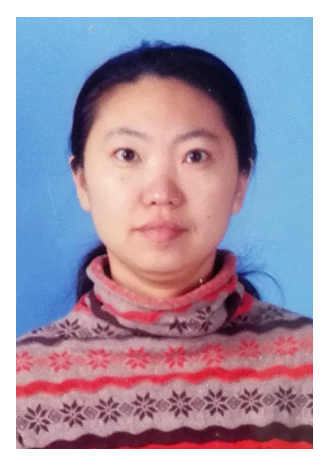
\includegraphics[width=1in,height=1.25in,clip,keepaspectratio]{author2_cdj.eps}}]{Danjie Chen} was now a lecturer in Huaqiao University, Xiamen, China. She received her M.S. degree in Computer Software from Beijing University of Technology. Her research interests include cooperative communication, cognitive radio networks.
\end{IEEEbiography}

% if you will not have a photo at all:
% insert where needed to balance the two columns on the last page with
% biographies
%\newpage

\begin{IEEEbiography}[]{Shaobin Cai} was now a Professor in Huaqiao University. He was a Post Doctor of computer department, UCLA, Member of China Computer Federation. His primary research interests include ad hoc networks, wireless sensor network, and underwater acoustic sensor network.
\end{IEEEbiography}

\begin{IEEEbiography}[{\includegraphics[width=1in,height=1.25in,clip,keepaspectratio]{author4_whc.eps}}]{Hsiao-Chun Wu} (M'00-SM'05-F'15) received a B. S. E. E. degree from National Cheng Kung University, Taiwan, in 1990, and the M. S. and Ph. D. degrees in electrical and computer engineering from University of Florida, Gainesville, in 1993 and 1999 respectively. From March 1999 to January 2001, he had worked for Motorola Personal Communications Sector Research Labs as a Senior Electrical Engineer. Since January 2001, he has joined the faculty in Department of Electrical and Computer Engineering, Louisiana State University, Baton Rouge, Louisiana, USA. From July to August 2007, Dr. Wu had been a visiting assistant professor at Television and Networks Transmission Group, Communications Research Centre, Ottawa, Canada. From August to December 2008, he was a visiting associate professor at Department of Electrical Engineering, Stanford University, California, USA.

Dr. Wu has published more than 120 peer-refereed technical journal and conference articles in electrical and computer engineering. His research interests include the areas of wireless communications and signal processing. He currently serves as an Associate Editor for IEEE Transactions on Broadcasting, IEEE Signal Processing Letters, IEEE Communications Magazine, etc. He used to serve as an Associate Editor for IEEE Transactions on Vehicular Technology. He has also served for numerous textbooks, IEEE/ACM conferences and journals as the technical committee, symposium chair, track chair, or the reviewer in signal processing, communications, circuits and computers.
\end{IEEEbiography}


% You can push biographies down or up by placing
% a \vfill before or after them. The appropriate
% use of \vfill depends on what kind of text is
% on the last page and whether or not the columns
% are being equalized.

%\vfill

% Can be used to pull up biographies so that the bottom of the last one
% is flush with the other column.
%\enlargethispage{-5in}

% that's all folks
\end{document}


